%\documentclass[11pt, a4paper]{article}
\documentclass[]{vgtuef}
%\usepackage[left=25mm,right=15mm,top=15mm,bottom=15mm]{geometry}
\usepackage[utf8x]{inputenc}
\usepackage[L7x]{fontenc}
\usepackage[lithuanian]{babel}
\usepackage{url}
\usepackage{float}
\usepackage{graphicx}
\usepackage{amsmath}
\usepackage{fancyhdr}
\usepackage{datetime}
\graphicspath{{img/}}
\usepackage{tikz}
\usepackage{gensymb}
\usepackage{epstopdf}
\renewcommand{\baselinestretch}{1.5}
\usepackage{subfig} 
%\usepackage{lastpage}
\usepackage{pgfplots}
%\usepackage{afterpage}
%\usetikzlibrary{arrows}
\usetikzlibrary{shapes.geometric, arrows}

\tikzstyle{startstop} = [rectangle, rounded corners, minimum width=3cm, minimum height=1cm,text centered, draw=black, fill=white]
\tikzstyle{process} = [rectangle, minimum width=3cm, minimum height=1cm, text centered, draw=black, fill=white]
\tikzstyle{io} = [trapezium, trapezium left angle=70, trapezium right angle=110, minimum width=3cm, minimum height=1cm, text centered, draw=black, fill=white]
\tikzstyle{decision} = [diamond, minimum width=3cm, minimum height=1cm, text centered, draw=black, fill=white]
\tikzstyle{arrow} = [thick,->,>=stealth]


\begin{document}

  \begin{titlepage}
    \begin{center}
      \includegraphics[width=58pt]{img/vgtu_logo.png}\\
      \textsc{\LARGE Vilniaus Gedimino Technikos universitetas}\\[1mm]
      \textsc{\Large Elektronikos fakultetas}\\[1mm]
      \textsc{\Large Elektroninių sistemų katedra}\\[40mm]
      \textsc{\Large Maksim NORKIN}\\[1mm]
      \textsc{\Large Objekto padėties nustatymas taikant MEMS jutiklius}\\[15mm]
      \textsc{\Large Investigation of the MEMS Sensor Based Object Position Estimation Methods}\\[10mm]
      \textsc{\large Magistro baigiamasis darbas}\\[10mm]
      \textsc{Informatikos inžinerijos studijų kryptis}\\
      \textsc{Informacinių elektroninių sistemų studijų programa, valst. kodas 621E15003}\\
      \textsc{Atvirojo kodo sistemų specializacija}\\
      \vfill
      {\large Vilnius, \the\year}
    \end{center}
  \end{titlepage}

  \newpage\null\thispagestyle{empty}\newpage

  \begin{titlepage}
    \setcounter{page}{7}
    \thispagestyle{plain}
    \begin{center}
      \textsc{\Large Vilniaus Gedimino Technikos universitetas}\\
      \textsc{\Large Elektronikos fakultetas}\\
      \textsc{\Large Elektroninių sistemų katedra}\\[10mm]
      \hfill
      \begin{minipage}{.35\linewidth}
        \begin{flushleft}
          \uppercase{Tvirtinu}\\
          Katedos vedėjas\\[5mm]
          \makebox[1.8in]{\hrulefill}\\
          \scriptsize{\textit{(parašas)}}\\
          \normalsize{\the\year m. \makebox[0.45in]{\hrulefill} mėn. \makebox[0.15in]{\hrulefill} d.}\\
        \end{flushleft}
      \end{minipage}\\[10mm]
      \textsc{\Large Maksim NORKIN}\\[1mm]
      \textsc{\Large Objekto padėties nustatymas taikant MEMS jutiklius}\\[15mm]
      \textsc{\Large Investigation of the MEMS Sensor Based Object Position Estimation Methods}\\[10mm]
      \textsc{\large Magistro baigiamasis darbas}\\[10mm]
      \textsc{Informatikos inžinerijos studijų kryptis}\\
      \textsc{Informacinių elektroninių sistemų studijų programa, valst. kodas 621E15003}\\
      \textsc{Atvirojo kodo sistemų specializacija}\\
    \end{center}
    \begin{flushright}
      \begin{minipage}[t]{.17\linewidth}
          \textbf{Vadovas}\\[3mm]
          \textbf{Konsultantas}
      \end{minipage}
      \begin{minipage}[t]{.4\linewidth}
        doc. dr. Raimondas Pomarnacki \\
        \scriptsize{\textit{(mokslinis vardas ir laipsnis, vardas, pavardė)}} \\
        \normalsize{dr. Aušra Žemienė} \\
        \scriptsize{\textit{(mokslinis vardas ir laipsnis, vardas, pavardė)}} \\
      \end{minipage}
      \begin{minipage}[t]{0.15\textwidth}
        \makebox[0.9in]{\hrulefill}\\
        \scriptsize{\textit{(parašas)}} \\
        \makebox[0.9in]{\hrulefill}\\
        \scriptsize{\textit{(parašas)}} \\
      \end{minipage}
      \begin{minipage}[t]{0.03\textwidth}
        \makebox[0.45in]{\hrulefill}\\
        \scriptsize{\textit{(data)}} \\
        \makebox[0.45in]{\hrulefill}\\
        \scriptsize{\textit{(data)}} \\
      \end{minipage}
    \end{flushright}
    \vfill
    \begin{center}
      {\large Vilnius, \the\year} 
    \end{center}
  \end{titlepage}

  \newpage\null\thispagestyle{empty}\newpage

  \setcounter{page}{9}

  %Anotacija
  Maksim NORKIN

Objekto padėties nustatymas taikant MEMS jutiklius. 
Magistro baigiamasis darbas informatikos inžinerijos laipsniui. 
Vilniaus Gedimino technikos universitetas.
Vilnius \the\year, TODO p. TODO iliustracijų, lentelių, bibliotekų, priedų.

Darbo tikslas yra sukurti objekto padėties nustatymo sistemą, taikant MEMS jutiklius ir mikrovaldiklį.
Pradžioje yra išnagrinėjami esami įgyvendinti funkcionalumai ir apibrėžiama, kokie šiuo metu yra taikomi sprendimai uždaviniui spręsti.
Atlikus analizę, sudarytas darbo planas išnagrinėti tris filtrus -- tiesinį (angl. \textit{linear}), išplėstinį (angl. \textit{extended}) ir sekamą (angl. \textit{unscented}) Kalman filtrus.
Išplėstas Kalman filtras industrijoje yra taikomas kaip standartas navigacinėse sistemose, sprendžiant netiesinio tipo uždavinius.
Visi trys filtrai buvo įgyvendinti ,,Matlab'' aplinkoje ir atliktas filtrų rezultatų palyginimas.
Buvo nustatyta -- blogiausiai netiesinį filtravimą atlieka tiesinis Kalman filtras, geriausiai - sekamas Kalman filtras.
Labai arti buvo išplėstas ir sekamas Kalman filtrai.
Po atliktos analizės sekamas Kalman filtras buvo įgyvendintas mikrovaldiklyje STM32.
  
  \newpage
  \newpage\null\thispagestyle{empty}\newpage

  \tableofcontents

  \newpage

  \section*{ĮVADAS}
  \addcontentsline{toc}{section}{ĮVADAS}

  Objekto padėties nustatymas turi dvi plačias pritaikymo sritis: inercinė navigacinė ir žmogaus judesio sekimo sistema \cite{schlomer2008gesture};

Objekto pozicijos nustatymas, panaudojus inercinius jutiklius remiasi prielaida, jog objektas lieka ramybės būsenoje tol, kol jį nepaveikia išorinė jėga. Tokia jėga suteikia objektui pagreitį. Jeigu rasta pagreitį galima išmatuoti ir suintegruoti, pagreičio ir pozicijos kitimas gali būti išmatuoti. Reikia nepamiršti, kad tokiu atveju matavimą sudarys dvi komponentės -- pagreitis dėl gravitacijos ir išorinės veikiančios jėgos pagreitis. Norint pašalinti gravitacijos komponentę iš pagreičio matavimo, reikia žinoti kokiu kampu akcelerometras yra vertikalės atžvilgiu.
Tokio kampo matavimui, reikalingas kitas jutiklis, kuris vadinasi giroskopas. Jis matuoja kampo greitį, kurį matematiškai integruojant, galima rasti kampo greičio pokytį nuo pradinio, žinomo kampo \cite{sukkarieh2000low}.

Akcelerometras suteikia pagreičio matavimą norimam objektui. Dažniausiai tokie matavimai yra užrašomi $x$, judėjimą tiesiai, $y$, šonu ir $z$ vertikaliai. Giroskopas suteikia matavimus, kurie dengia nurodytas ašis ir yra užrašomi $\theta$, sūkiui, $\beta$ polinkiui ir $\gamma$ vingiavimui, kaip pavaizduota \ref{tikz:axis_of_the_system} pavyzdyje. Tokių inercinių įverčių naudojimas turi pagrindinį privalumą -- stebimo objekto polinkis ir pagreitis gali būti vertinami bet kokioje navigacijoje.  

\begin{figure}[H]
    \centering
    \caption{Objekto pozicijos pagreičio pokyčio ašys, $x$, $y$ ir $z$. Sūkio matmenys apie ašis $\theta$, $\beta$ ir $\gamma$.}
    \label{tikz:axis_of_the_system}
    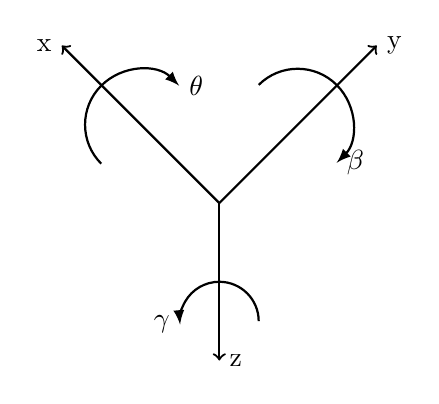
\begin{tikzpicture}
        % axis
        \draw[thick, black, ->] (0,0) -- ( 2, 2) node [right] {y};
        \draw[thick, black, ->] (0,0) -- (-2, 2) node [left] {x}; 
        \draw[thick, black, ->] (0,0) -- ( 0,-2) node [right] {z};
        % arc
        \draw[thick, -latex] ( 0.5,  1.5) arc (135:-45:0.70) node [right] {$\beta$}; 
        \draw[thick, -latex] (-1.5,  0.5) arc (225:45:0.70) node [right] {$\theta$};
        \draw[thick, -latex] ( 0.5, -1.5) arc (0:185:0.5) node [left] {$\gamma$};
    \end{tikzpicture}
\end{figure}

Inercinės navigacijos sistemos yra naudojamos labai plačiai lėktuvuose, raketose, kosmoso laivuose, povandeniniuose ir vandens laivuose \cite{woodman2007introduction}. Progresas gaminant MEMS įrenginius, sudarė galimybes kurti mažas ir lengvas navigacines sistemas. Tokie privalumai leidžia praplatinti įrenginių panaudojimo galimybes ir šiuo metu įtraukia tokias sritis kaip žmogaus ir gyvūnų judesio sekimą.

Tačiau reikia nepamiršti ir apie klaidas, kurias sukelia nuolatinė dedamoji, santykio įverčiai ir nelinijines sistemos įtakos jutiklio verčių nuskaitymo metu. Tokios klaidos yra pagrindinė priežastis atsirasti netikslumams navigacinėje sistemoje per laiko vienetą. Netikslumai sąlygoja akselerometro įverčius, kuriuos tampa labai sunku atskirti tarp gravitacinio lauko ir objekto judėjimo, ko pasekoje objekto pozicijos matavimas toliau yra dar netikslesnis. Kadangi inerciniai jutikliai yra tokio tipo, kuriems yra labai svarbi tiksli prieš tai buvusi pozicija, bet kokia klaida skaičiuojant prieš tai buvusia pozicija, įtakoja ir dabartinės pozicijos skaičiavimą. Tokiu būdu, su laiku navigacinė sistema tampa visiškai netiksli ir praranda visą savo vertę.

  \section{APŽVALGA}

  Šiame skyriuje apžvelgti MEMS pagreičio ir giroskopo tipo jutikliai. 
Aptariama, kokie yra didžiausi jų privalumai ir trūkumai (didelis duomenų triukšmas ir būdai jiems kompensuoti ar mažinti).

\subsection{Giroskopas}

MEMS tipo jutiklis \cite{perlmutter2012high} yra gaminamas staklėmis iš silikono mikro-apdorojimo būdu, turi labai mažai dalių, o jo gamybos kaštai yra gana maži.

MEMS giroskopai yra veikiami \textit{Coriolio efekto}, kuris sako, jog turint koordinačių ašį, sukantis kampiniu greičiu $w$, objektas su mase $m$, kuris juda greičiu $v$, yra veikiamas jėgos

\begin{equation}
    F_c = -2m(w \times v)
\end{equation}

MEMS giroskopai susideda iš vibracinės kilmės elementų, kurie yra naudojami matuojant \textit{Coriolio} efektą. 
Egzistuoja labai daug vibracinių geometrijų, tarp kurių yra vibracinis ratas ir kamertono giroskopai. 
Paprasčiausia geometrija susideda iš vienos masės, kuri skirta vibruoti viena ašimi. 
Kai tik giroskopas yra pasukamas, įvedama antrinė vibracija statmenai pirminei ašiai dėl \textit{Coriolis} jėgos. 
Dėl to, kampinis greitis gali būti apskaičiuojamas, matuojant antrinį apsisukimą. 
Šiuo metu MEMS jutikliai negali pasiekti tokio tikslumo lygio, kokį siūlo optiniai jutikliai, tačiau yra tikimasi, kad ateityje MEMS jutikliai tikslumu nebus prastesni nei optiniai jutikliai.

MEMS jutikliai turi labai daug privalumų, palyginti su kitais jutikliais \cite{titterton2004strapdown}:

\begin{itemize}
    \item mažas dydis;
    \item mažas svoris;
    \item patvari konstrukcija;
    \item mažos galios naudojimas;
    \item labai greitas paleidimo laikas;
    \item pigi gamyba, esant dideliam mastui;
    \item patikimi;
    \item reikalauja labai mažai priežiūros;
    \item gali būti naudojami sudėtingomis sąlygomis;
\end{itemize}

\subsubsection{Nuolatinė dedamoji}

Vidutinis kampo pokyčio matavimas, palaikant visišką giroskopo ramybės būseną, yra laikomas nuolatine giroskopo dedamąja. 
Matuojama yra $\degree/h$. 
Nuolatinės dedamosios klaida $\epsilon$ yra apskaičiuojama integruojant ir priklauso nuo laiko $\theta(t) = \epsilon \cdot t$.

Klaida gali būti nustatyta, panaudojus labai ilgo laikotarpio vidutinę vertę, kuomet giroskopas yra paliktas visiškos ramybės būsenos ir nėra veikiamas jokių išorinių jėgų. 
Kai tik nuolatinė dedamoji yra žinoma, labai yra svarbu ją kompensuoti tikro matavimo metu.

\subsubsection{Atsitiktinis kampinis pokytis}

Jutiklio vertės matavimo metu yra galimas triukšmas, sukeliamas terminių ir mechaninių trukdžių, kurių dažnis yra žymiai didesnis už jutiklio vertės matavimo dažnį.
Tokių veiksnių rezultatas yra signalas, kuriame yra balto triukšmo. 
Tai yra paprasčiausia eilė skaičių, kurių vidurkis lygus nuliui.
Nėra jokios koreliacijos ir yra visiškai atsitiktiniai skaičiai. 
Tokiu būdu kiekvienas atsitiktinis skaičius yra tolygiai paskirstytas ir turi baigtinį $\sigma^2$ pasiskirstymą.

Net ir neišvedus formulės (detalus išvedimas yra pateikiamas \cite{woodman2007introduction}) galima teigti, jog triukšmas įveda ,,atsitiktinio vaikščiojimo'' (angl. \textit{random walk}) klaidą integraliniame signale, kuri yra nulinio vidurkio ir kurios variacija didėja nuo laiko pokyčio šaknies.
\begin{equation}
    \sigma_{\theta} (t) = \sigma \cdot \sqrt{ \delta t \cdot t}
\end{equation}
Čia $\sigma$ yra triukšmo signalo pokytis, $t$ yra visas jutiklio įverčio nuskaitymo periodas, o $\delta t$ yra laiko skirtumas tarp nuskaitymų.

Kadangi dominantis įvertis yra kaip triukšmas, lemiantis integralinį signalą, labai dažnai gamintojai nurodo gaminamo jutiklio atsitiktinį kampinį pokytį. Jis yra žymimas $\degree/\sqrt{h}$. 
Pavyzdžiui, jeigu jutiklis yra $0,3\degree / \sqrt{h}$, tai reiškia, jog po vienos valandos standartinės variacijos pozicijos orientacijos klaida sudarys $0,3\degree$, po dviejų valandų $\sqrt{2} * 0,3 = 0.42 \degree$.

\subsection{Nuolatinės dedamosios stabilumas}

Nuolatinė dedamoji MEMS giroskope keičiasi laikui bėgant dėl virpėjimo triukšmo elektronikos ir kituose įtaisuose, kurie potencialiai gali būti paveikti atsitiktinio virpėjimo. 
Virpėjimo triukšmas yra $1/f$ spektro, kurio efektai yra pastebimi elektroniniuose komponentuose, esant žemiems dažniams. 
Esant aukštiems dažniams virpėjimas yra uždengiamas balto triukšmo. 
Nuolatinės dedamosios nestabilumas, kuris kyla dėl virpėjimo, dažniausiai yra modeliuojamas kaip atsitiktinis kampinis pokytis.

Nuolatinės dedamosios stabilumo įvertis nurodo, kiek gali keistis per fiksuotą laiko tarpą. 
Dažniausiai imamas $100~s$ laiko rėžis, kuomet aplinka visiškai nesikeičia. 
Įvertis žymimas kaip $1\sigma$ ir matuojamas $\degree/h$ arba $\degree/s$, kai įranga yra labai netiksli. 
Nuolatinės dedamosios stabilumas yra modeliuojamas atsitiktinio vaikščiojimo procesu. 
Tai galima interpretuoti turint $B_t$ kaip dedamosios vertė laiku $t$, tuomet $1\sigma$ stabilumas $0,01\degree/h$ per 100 sekundžių reiškia, kad dedamoji laiku $t+100$ yra atsitiktinis skaičius, kurio vertė yra tikėtina $B_t$ su $0,01\degree/h$ variacija. 
Po tam tikro laiko, variacija sukuria atsitiktinį vaikščiojimą, kurio nuokrypis didėja per laiko vieneto šaknį. 
Dėl šitos priežasties nuolatinės dedamosios stabilumas yra žymimas kaip dedamosios atsitiktinis vaikščiojimo matas

\begin{equation}
    BRW (\degree / \sqrt{h}) = \frac{BS(\degree/h)}{\sqrt{t(h)}},
\end{equation}
kur $t$ yra nuolatinės dedamosios stabilumo laikas.

Praktikoje yra truputį kitaip. 
Jeigu stabilumas būtų modeliuojamas kaip atsitiktinis vaikščiojimas, tai integracinis įverčio skaičiavimas smarkiai padidintų klaidos įvertį. 
Dėl to, yra nutarta nustatyti rėžius, kuriuose yra nurodomas stabilumas.

\subsubsection{Temperatūros efektai}

Temperatūros svyravimai kyla dėl aplinkos temperatūros nepastovumo ir pačio jutiklio temperatūros nepastovumo. 
Tokie svyravimai natūraliai įtakoja ir nuolatinę dedamąja. 
Jie visiškai nėra nurodomi nuolatinės dedamosios klaidos skaičiavimuose.

Bet koks likutinis nuolatinės dedamosios įterpimas dėl temperatūros pokyčio smarkiai padidins įverčio klaidą ir klaida laikui bėgant didės.
Santykis MEMS jutikliuose tarp temperatūros ir klaidos yra netiesinis.
Dauguma inercinių matavimo sistemų turi savo viduje temperatūros daviklį, todėl matavimo klaidą galima kompensuoti tokiu būdu. 
Kai kurios matavimo sistemos siūlo automatinį klaidos taisymą.

\subsubsection{Kalibravimo klaidos}

Kalibravimo klaidų terminas susieja grupę klaidų šaltinių, kurie susideda iš santykio faktoriaus, lygiavimo ir giroskopų tiesiškumo. 
Tokio tipo klaidų galima pastebėti tik išoriškai veikiant jutiklį ir stebint nuolatinės dedamosios pokytį. 
Tai sukelia integracinio signalo netikslumų, prie kurių prisideda papildomi svyravimai, kurių dydis yra santykis tarp pokyčio ir vykdymo laiko. 
Dažniausiai tokio tipo klaidas galima išmatuoti ir jas kompensuoti.

% Akcelerometras

\subsection{Pagreičio jutiklis}

Mikro-staklių pagaminti silikoniniai pagreičio jutikliai naudoja tokius pačius principus, kaip ir mechaniniai ar kietieji jutikliai. 
Egzistuoja du pagrindiniai MEMS pagreičio jutiklių tipai. 
Pirmas tipas yra mechaniniai pagreičio jutikliai, kurie yra pagaminti iš silikono. 
Jie veikia lygiai tokiais pačiais principais, kaip ir mechaniniai jutikliai. 
Antras jutiklių tipas - kurie matuoja vibracijos pokyčius vibraciniam elemente, ko pasekoje yra stebimi įtampos pokyčiai.

Pagreičio MEMS jutiklių privalumai yra lygiai tokie patys, kaip ir MEMS giroskopinių jutiklių. 
Taip pat, pagrindinis tokių jutiklių minusas prieš kito gaminimo tipo jutiklius - mažas tikslumas. 

\subsubsection{Nuolatinė dedamoji}

Vertės dedamoji, pagreičio matavimo jutiklyje, yra skirtumas tarp matuojamos vertės ir realios vertės, matuojama $m/s^2$.
Pastovios dedamosios klaida $\epsilon$, po dvigubos integracijos, sukuria klaidą, kuri laikui bėgant didėja keturis kartus. 
Sukaupta klaida, priklausomai nuo pozicijos yra

\begin{equation}
    s(t) = \epsilon \cdot \frac{t^2}{2},
\end{equation}
kur $t$ yra integravimo laikas.

Yra galimybių vertinti dedamąją atliekant matavimus su duotu jutikliu labai ilgą laiką, kuriuo neveikia jokia išorinė jėga. 
Deja, visiškai izoliuoti jutiklio nėra galima, kadangi iškarto erdvėje pradeda veikti gravitacija, kuri veikia jutiklį, patiekdama savo nuolatinę dedamąja. 
To pasekoje, labai svarbu yra žinoti įrenginio pozicija žemės atžvilgiu, iš kurios pusės veikia gravitacinė jėga. Praktikoje tai yra pasiekiama naudojant kalibravimo procedūra, kurios metu įrenginys yra pritvirtinamas prie paviršiaus, kurio orientacija gali būti kontroliuojama labai tiksliai.

\subsubsection{Atsitiktinis pagreičio pokytis}

Pagreičio MEMS jutiklio išėjimo matavimai yra veikiami balto triukšmo. 
Kaip jau buvo paminėta giroskopo atsitiktinio kampo pokyčio poskyryje, balto triukšmo integracija sudaro sąlygas variacijai didėti proporcingai $\sqrt{t}$. 
To pasekoje, jutiklio išėjime yra stebimas atsitiktinis verčių vaikščiojimas, kuris vertinamas $m/s/\sqrt{h}$. Praleidžiant standartinės variacijos išvedimą, kuris yra aprašytas \cite{woodman2007introduction}, galima iškarto teigti, kad pagreičio jutiklio baltas triukšmas sukuria antro lygio atsitiktinį verčių vaikščiojimą pozicijoje, su vidurkiu, kuris lygus nuliui ir standartiniu nuokrypiu

\begin{equation}
    \sigma_{s}(t) \approx \sigma \cdot t^{3/2} \cdot \sqrt{\frac{\delta t}{3}},
\end{equation}
kuris didėja proporcingai nuo $t^{3/2}$. 
Čia $t$ yra visas matavimo laikas, $\delta t$ yra skirtumas tarp įverčio matavimo laikų.

\subsubsection{Vibraciniai triukšmai}

MEMS tipo pagreičio jutikliai yra veikiami vibracijos triukšmo, kuris sukelia nuolatinės dedamosios stabilumo klaidą per laiką. 
Tokie nukrypimai yra dažnai modeliuojami kaip nuolatinės dedamosios atsitiktiniai judėjimai, kaip jau buvo aprašyta giroskopo atveju. 
Naudojantis tokiu modeliu, vibracijos sukuria antro lygio atsitiktinio vaikščiojimo triukšmą pagreičiui, proporcingai $t^{3/2}$ ir trečio lygio atsitiktinį vaikščiojimą, kuris yra proporcingas $t^{5/2}$.

\subsubsection{Temperatūros efektai}

Kaip ir giroskopu atžvilgiu, temperatūros pokyčiai įtakoja vibracinius pokyčius, kas sukelia dedamosios nestabilumus išėjimo signale. 
Dedamosios santykis su temperatūra labai priklauso nuo įrangos, tačiau dažniausiai jis yra ne linijinis. 
Bet koks liekamasis nuolatinės dedamosios komponentas sukelia klaida, kuri didėja keturgubai bėgant laikui. 
Pagreičio jutiklio korekcijos dėl temperatūros kai kurie matavimo įrenginiai automatiškai kompensuoja.

\subsubsection{Kalibravimo klaidos}

Kalibravimo klaidos atsiranda kaip nuolatinės dedamosios klaidos. 
Jie pasirodo įverčiuose tik tuomet, kai jutiklis yra veikiamas kažkokio pagreičio jėgos. 
Taip pat verta stebėti gravitaciją, kadangi ji gali sukelti tokias laikinas klaidas ir tuomet, kai jutiklis yra pastovioje pozicijoje ir nėra veikiamas išorinės pagreičio jėgos.



  Šiame skyriuje apžvelgti pagrindiniai signalų filtravimo įrankiai, kurie yra plačiai naudojami inercinėse navigacinėse sistemose.

\subsection{Kalman filtras}

    Kalman filtras \cite{kalman1960new} yra vienas iš labiausiai naudojamų duomenų sujungimo algoritmų informacijos apdorojimo pramonės srityje \cite{faragher2012understanding}. Pats žymiausias Kalma filtro panaudojimas jo ankstyvoje stadijoje yra \textit{Apollo} navigaciniam kompiuteryje, kuris nugabeno \textit{Neil Armstrong} iki mėnulio ir svarbiausia -- atgal. Šiais laikais, Kalman filtrą galima rasti beveik kiekviename įrenginyje -- mobiliam telefone, kompiuteriniuose žaidimuose.

    \subsubsection{Diskretaus laiko Kalman filtras}

    Tarkime, kad turime linijinę diskretaus laiko sistemą

    \begin{equation}
        x_k = F_{k-1}x_{k-1} + G_{k-1}u_{k-1} + w_{k-1}
    \end{equation}
    \begin{equation}
        y_k = H_k x_k + v_k
    \end{equation}

    Proceso triukšmai ${w_k}$ ir ${v_k}$ yra baltas, nulinio vidurkio, be koreliacijos ir žinomos kovariacijos matricos

    \begin{equation}
    w_k \sim (0, Q_k)
    \end{equation}
    \begin{equation}
    v_k \sim (0, R_k)
    \end{equation}
    \begin{equation}
    E[w_k w_j^T] = Q_k \delta_{k-j}
    \end{equation}
    \begin{equation}
    E[v_k v_j^T] = R_k\delta_{k-j}
    \end{equation}
    \begin{equation}
    E[v_k w_j^T] = 0,
    \end{equation}

    kur $\delta_{k-j}$ yra Kroneckerio delta funkcija, $\delta_{k-j} = 1$, jeigu $k=j$ ir $\delta_{k-j} = 0$, kai $k \neq j$.
    Tikslas yra spėti $x_k$ būsena, remiantis žiniomis apie sistemos dinamikas ir turimu mėginiu, kuris yra triukšmingas ${y_k}$.
    Informacijos kiekis, kuris yra galimas spėjimui skiriasi nuo problemos, kuria yra norima išspręsti.
    Jeigu egzistuoja visi mėginiai, iki laiko $k$, kuriuos galima panaudoti $x_k$ spėjimui, galima suformuoti tolesnį spėjimą, kuri galima pažymėti kaip $\hat{x}_k^{+}$.
    Ženklas $+$ reikia, kad spėjimas yra tolimesnis.
    Vienas iš būdu kaip galima suformuoti tolimesnę būseną yra apskaičiuoti spėjamą $x_k$ vertę, kuri priklauso nuo turimų mėginių iki laiko $k$:

    \begin{equation}
        \hat{x}_k^{+} = E[x_k|y_1,y_2, \dots , y_k]
    \end{equation}

    Jeigu turimi visi matavimai prieš (ir neįtraukiant) laiką $k$ naudojimui, tuomet galima suformuluoti ankstesnį spėjimą, kuris yra žymimas kaip $\hat{x}_k^{-}$.
    Pagalbinis žymėjimas $-$, reiškia ankstesnį spėjimą.
    Vienas iš būdų suformuluoti ankstesnį spėjimą yra apskaičiuoti $x_k$ vertę, kuri priklauso nuo visų turimų matavimų prieš laiką $k$:

    \begin{equation}
        \hat{x}_k^{-} = E[x_k|y_1,y_2,\dots, y_{k-1}]
    \end{equation}

    Labai svarbu pažymėti, jog $\hat{x}^-_k$ ir $\hat{x}_k^{+}$ abu kartu yra spėjimai tokio pačio lygumo; jie abu yra $x_k$ spėjimai.
    Tačiau, $\hat{x}_k^-$ yra $x_k$ spėjimas prieš $y_k$ matavimą, o $\hat{x}_k^+$ yra spėjimas po to, kai $y_k$ matavimas yra atliktas.
    Natūraliai yra tikimąsi, jog $\hat{x}_k^+$ bus geresnis spėjimas už $\hat{x}_k^-$, kadangi tuo metu yra daugiau informacijos skaičiuojant $\hat{x}_k^+$:

    \begin{enumerate}
        \item $\hat{x}_k^-$ = $x_k$ spėjimas prieš mėginio gavimą laiku $k$
        \item $\hat{x}_k^+$ = $x_k$ spėjimas, po mėginio gavimo laiku $k$
    \end{enumerate}

    Jeigu egzistuoja mėginiai po laiko $k$, kuriuos galima naudoti $x_k$ spėjimui, tuomet galima suformuoti glotnesnį spėjimą.
    Vienas iš būdų suformuoti glotnesnį spėjimą yra apskaičiuoti tikėtiną $x_k$ vertę, kuri priklauso nuo visų turimų įverčių

    \begin{equation}
        \hat{x}_{k|k+N} = E[x_k|y_1,y_2,\dots,y_k,\dots, y_{k+N}],
    \end{equation}
    kur $N$ yra teigimas skaičius, kurio vertė priklauso nuo specifinės problemos, kuri yra sprendžiama.
    Jeigu galima rasti geriausią $x_k$ spėjimą daugiau negu vienu žingsniu greičiau už turimus mėginius, galima suformuluoti spėjamą būseną.

    \begin{equation}
        \hat{x}_{k|k-M} = E[x_k|y_1,y_2, \dots, y_{y-M}],
    \end{equation}
    kur $M$ yra teigiamas skaičius, kurio vertė priklauso nuo sprendžiamo uždavinio.

    Tolimesniam žymėjime bus pateiktas $\hat{x}_0^+$ įvertis, kuris parodys pradinį $x_0$ įvertinimą prieš bet kokius turimus mėginius.
    Pirmas mėginys yra gaunamas laiku $k=1$.
    Kadangi neegzistuoja jokie mėginiai, kuriuos galima panaudoti spėti $x_0$, yra logiška suformuoti $\hat{x}^+_0$ kaip pradinės būsenos $x_0$ tikėtiną įvertį:

    \begin{equation}
        \hat{x}_0^+ = E(x_0)
    \end{equation}

    Spėjimo klaidos kovariacijos matricai pažymėti bus panaudotas $P_k$ žymėjimas.
    $P_k^-$ žymi $\hat{x}_k^-$ įvertinimo klaidos kovariaciją, o $P_k^+$ žymi $\hat{x}_k^+$ įvertinimo klaidą.

    \begin{equation}
        P_k^- = E[(x_k - \hat{x}_k^-)(x_k - \hat{x}_k^-)^T]
    \end{equation}
    \begin{equation}
        P_k^+ = E[(x_k - \hat{x}_k^+)(x_k-\hat{x}_k^+)^T]
    \end{equation}

    Po to, kai yra apdorotas įvertis laike $(k-1)$, gaunamas $x_{k-1}$ įvertinimas (žymimas $\hat{x}_{k-1}^+$) ir įverčio kovariacijos matrica (žymima $P_{k-1}^+$).
    Kai ateina laikas $k$, prieš apdorojant įverčiui laike $k$, apskaičiuojame $x_k$ įvertį (žymima $\hat{x}_k^-$) ir įverčio klaidos kovariacijos matricą (žymima $P_k^-$).
    Tuomet yra apdorojamas gautas įvertis laike $k$ ir patobuliname įvertį $x_k$.
    Gautas galutinis įvertis $x_k$ yra žymimas $\hat{x}_k^+$, o jo kovariacijos matrica $P_k^+$.

    Spėjimo procesas pradedamas nuo $\hat{x}_0^+$, geriausiai žinomos pradinės $x_0$ būsenos.
    Turint $\hat{x}_0^+$, kaip apskaičiuoti $\hat{x}_1^-$?
    Reikia prilyginti $\hat{x}_1^- = E(x_1)$.
    Reikia pažymėti, jog $\hat{x}_0^+ = E(x_0)$, ir prisiminti, kad $x$ vidurkis kinta laike

    \begin{equation}
        \bar{x}_k = F_{k-1}\bar{x}_{k-1} + G_{k-1}u_{k-1}
    \end{equation}

    Tokiu atveju gaunama

    \begin{equation}
        \hat{x}_1^- = F_0\hat{x}_0^+ + G_0u_0
    \end{equation}

    Šita lygtis yra specifinė lygtis, kuri rodo kaip gauti $\bar{x}_1^-$ iš $\bar{x}_0^+$. Labiau bendrinant, gaunama lygtis

    \begin{equation}
        \hat{x}_k^- = F_{k-1}\bar{x}_{k-1}^+ + G_{k-1}u{k-1}
    \end{equation}

    Ir jinai yra vadinama $\bar{x}$ laiko atnaujinimo lygtis.
    Nuo laiko $(k-1)^+$ iki laiko $k^-$, būsenos įvertis kinta tokiu pačiu principu, kaip ir būsenos vidurkis.
    Neegzistuoja jokios papildomos informacijos, kuri leistu atnaujinti būseną tarp laiko $(k-1)^+$ ir $k^-$, todėl reikia tiesiog atnaujinti būsenos įvertį, remiantis sistemos dinaminėmis žiniomis.

    Toliau reikia apskaičiuoti laiko atnaujinimo $P$ lygtį.
    Pradedama nuo $P_0^+$, kuris žymi pradinės būsenos įverčio $x_0$ kovariaciją.
    Jeigu labai gerai yra žinoma apie pradinę sistemos būseną, tuomet $P_0^+ = 0$.
    Jeigu visiškai nėra aišku apie pradinę sistemos būseną, tuomet $P_0^+ = \inf$.
    Bendrai, $P_0^+$ parodo pradinės $x_0$ būsenos neužtikrintumą

    \begin{equation}
        P_0^+ = E[(x_0 - \hat{x}_0^+)(x_0 - \hat{x}_0^+)^T]
    \end{equation}

    Turint $P_0^+$, kaip apskaičiuoti $P_1^-$? Reikia prisiminti kaip linijinės diskretaus laiko būsenos kovariacija kinta su laiku ir gaunam

    \begin{equation}
        P_1^- = F_0 P_0^+F_0^T + Q_0
    \end{equation}

    Tai yra specifinė lygtis, o bendresnė lygtis atrodo taip

    \begin{equation}
        P_k^- = F_{k-1}P_{k-1}^+F_{k-1}^T + Q_{k-1},
    \end{equation}
    ir vadinama $P$ laiko atnaujinimo lygtimi.

    Aukščiau yra išvestos lygtis, kurios yra skirtos apskaičiuoti $\hat{x}$ ir $P$.
    Dabar reikalinga išvesti lygtis, kurios skirtos atnaujinti $\hat{x}$ ir $P$ po atlikto sistemos matavimo.
    Turint $\hat{x}_k^-$, kaip apskaičiuoti $\hat{x}_k^+$? Tiek $x_k^-$ ir $x_k^+$ yra $x_k$ įverčiai.
    Vienintelis skirtumas tarp $\hat{x}_k^-$ ir $\hat{x}_k^+$, kad $\hat{x}_k^+$ yra gaunamas turint mėginį $y_k$.
    Remiantis mažiausių kvadratų teorija, mėginys $y_k$ keičia $x$ konstantos spėjimą:

    \begin{equation}
        K_k = P_{k-1}H_k^T(H_kP_{k-1}H_k^T + R_k)^{-1} = P_kH_k^TR_k^-1
    \end{equation}
    \begin{equation}
        \bar{x}_k = \bar{x}_{k-1} + K_k(y_k - H_k\bar{x}_{k-1})
    \end{equation}
    \begin{equation}
        P_k = (I - K_kH_k)P_{k-1},
    \end{equation}
    kur $\bar{x}_{k-1}$ ir $P_{k-1}$ yra įvertinimas ir jo kovariacija prieš $y_k$ matavimą ir $\bar{x}_k$ ir $P_k$ yra įvertinimas ir jo kovariacija po $y_k$ matavimo.

    Atlikę porą pakeitimų, gauname

    \begin{equation}
        K_k = P_{k}^+H_k^TR_k^{-1}
    \end{equation}
    \begin{equation}
        \bar{x}_k^+ = \bar{x}_k^- + K_k(y_k - H_k\bar{x}_k^-)
    \end{equation}
    \begin{equation}
        P_k^+ = (I-K_kH_k)P_{k}^-
    \end{equation}

    Taip yra gaunamos lygtis, kurios yra naudojamos įverčiams $\bar{x}_k$ ir $P_k$ atnaujinti, po gauto mėginio.
    Matrica $K_k$ aukštesnėse lygtyse yra vadinama Kalmano augimu.

    \subsubsection{Pavyzdys}

    Geriau suprasti turimą teoriją, pateikiamas Niutono sistemos pavyzdys, kurioje nėra jokios triukšmo, su pozicija $r$, greičiu $v$ ir pastoviu pagreičiu $a$.
    Sistema galima apibūdinti kaip

    \begin{equation}
        \begin{bmatrix} \dot{r} \\ \dot{v} \\ \dot{a} \end{bmatrix} =
        \begin{bmatrix} 0 & 1 & 0 \\ 0 & 0 & 1 \\ 0 & 0 & 0 \end{bmatrix}
        \begin{bmatrix} r \\ v \\ a \end{bmatrix}
    \end{equation}
    \begin{equation}
        \dot{x} = Ax
    \end{equation}

    Diskretizuota sistemos versija (su diskretizacijos periodu $T$) yra užrašoma kaip\

    \begin{equation}
        x_{k+1} = Fx_k,
    \end{equation}
    kur $F$ yra duodamas kaip

    \begin{equation}
        F = exp(AT) = I + AT + \frac{(AT)^2}{2!} + \dots =
        \begin{bmatrix}
            0 & T & T^2/2 \\
            0 & 1 & T \\
            0 & 0 & 1
        \end{bmatrix}
    \end{equation}

    Kalmano filtras tokiai sistemai yra išreiškiamas

    \begin{equation}
        \bar{x}_k^- = F\bar{x}_{k-1}^+
    \end{equation}
    \begin{equation}
        P_k^- = FP_{k-1}^+ F^T + Q_{k-1} = FP_{k-1}^+ F^T
    \end{equation}

    Ką galima pastebėti, kad kovariacijos įverčio klaidos matrica didėja tarp laiko $(k-1)^+$ (laikas $(k-1)$, po kurio gautas įvertis yra apdorotas) ir $k^-$ (laikas $k$, prieš apdorojant gautą įvertį).
    Kadangi nėra gaunamas joks mėginys tarp laikų $(k-1)^+$ ir $k^-$, yra daug logikos, jog duota kovariacijos matrica didėja.
    Dabar galima įvesti triukšmą, kuris būtų mėginio gavimo triukšmas $\sigma^2$

    \begin{equation}
        y_k = H_kx_k + v_k = \begin{bmatrix} 1 & 0 & 0 \end{bmatrix} x_k + v_k
    \end{equation}
    \begin{equation}
        v_k ~ (0, R_k)
    \end{equation}
    \begin{equation}
        R_k = \sigma^2
    \end{equation}

    Kalmano augimas gaunamas kaip

    \begin{equation}
        K_k = P_k^-H_k^T(H_kP_k^-H_k^T+R_k)^{-1}
    \end{equation}

    Perrašius $P_k$ kaip trijų elementų vektorių

    \begin{equation}
        K_k = \begin{bmatrix} P_{k,11}^- \\ P_{k,12}^- \\ P_{k,13}^- \end{bmatrix} \frac{1}{P_{k,11}^- + \sigma^2}
    \end{equation}

    Tolimesnė kovariacija gaunama

    \begin{equation}
        P_k^+ = P_k^- - K_kH_kP_k^-
    \end{equation}

    Kai yra gaunamas naujas matavimas, yra natūraliai tikimąsi, jog būsenos spėjimas bus tikslesnis.
    Tai reiškia, jog kovariacija mažės, ką ir rodo lygtis.

    \subsection{Ištiesintas Kalman filtras}

    Šiame skyriuje parodoma kaip ištiesinti ne tiesinę sistemą ir tuomet panaudoti Kalman filtro teoriją įvertinant skirtumus tarp būsenos ir nominalios būsenos vertės.
    Toliau tai suteiks ne tiesinės sistemos būsenos įvertinimą.
    Ištiesintas Kalman filtras yra išvedamas iš nuolatinio laiko požiūrio, o diskretaus ar hibridinio laiko išvedimai yra analogiški.

    Tarkime, egzistuoja toks ne tiesinės sistemos modelis:

    \begin{equation}
        \dot{x} = f(x,u,w,t)
    \end{equation}
    \begin{equation}
        y = h(x,v,t)
    \end{equation}
    \begin{equation}
        w ~ (0,Q)
    \end{equation}
    \begin{equation}
        v ~ (o,R)
    \end{equation}

    Sistemos lygtis $f(\cdot)$ ir matavimo lygtis $h(\cdot)$ yra ne tiesinės funkcijos.
    Bus naudojama Tailoro eilutė išplėsti šitas lygtis aplink nominalią kontrolę $u_0$ ir nominalią būseną $x_0$ su $y_0$ išėjimu, bei triukšmu $w_0$ir $v_0$.
    Šios nominalios vertės yra paremtos ankstesniu spėjimu apie sistemos trajektoriją.
    Pavyzdžiui, jeigu sistemos lygtis pateikia lėktuvo dinamikas, tuomet nominali kontrolė, būsena ir išėjimas gali būti suplanuoto skrydžio trajektorija.
    Reali skrydžio trajektorija skirsis nuo šios nominalios trajektorijos dėl modeliavimo klaidos, trikdymų ir kitų nenumatytų efektų.
    Tačiau reali trajektorija turi būti arti nominalios trajektorijos, tokiu atveju Tailoro eilutės tiesinimas turi būti labai arti.
    Tailoro eilutės išskleidimas suteikia

    \begin{equation}
        \begin{aligned}
            \dot{x} &\approx f(x_0, u_0, w_0, t) + \frac{\delta f}{\delta x}\Bigr|_{0} (x-x_0) + \frac{\delta f}{\delta u}\Bigr|_{0} (u-u_0) + \frac{\delta f}{\delta w}\Bigr|_{0} (w-w_0) \\
            &= f(x_0, u_0, w_0, t) + A\Delta x + B \Delta u + L \Delta w
        \end{aligned}
    \end{equation}
    \begin{equation}
        \begin{aligned}
            y &\approx h(x_0, v_0, t) + \frac{\delta h}{\delta x}\Bigr|_{0}(x-x_0) + \frac{\delta h}{\delta v}\Bigr|_{0}(v-v_0) \\
            &= h(x_0, v_0, t) + C \Delta x + M \Delta v
        \end{aligned}
    \end{equation}

    Šie dalinių matricų A, B, C, L ir M išvestinės yra išskiriamos iš aukštesnių lygčių.
    Indeksas "0" rodo, kad dalinę išvestinę reikia atlikti esant nominaliai kontrolei, būsenai, išėjimui ir triukšmams.

    Galima padaryti prielaida, kad nominalaus triukšmo įverčiai yra abu lygus 0 šiuo atveju.
    Kadangi jie abu yra lygus 0, tuomet $\delta w(t) = w(t)$ ir $\delta v(t) = v(t)$.
    Toliau galima teigti, kad kontrolė $u(t)$ yra labai gerai žinoma.
    Bendru atveju, tai yra labai gera prielaida, kadangi kontrolės įėjimas $u(t)$ yra pateiktas sistemos kontrolės, kuri neturi turėti jokių abejonių įverčiuose.
    Tai reiškia, kad $u_0(t) = u(t)$ ir $\delta u(t) = 0$.
    Tačiau, realybėje gali būti neužtikrintumas kontrolės išėjime, kadangi jos yra sujungtos su kažkokiu įtaisu, kuris turi savo vidurkį ir triukšmą.
    Dabar galima aprašyti nominalios sistemos trajektoriją kaip

    \begin{equation}
        \label{eq:nominal_sistem_trajektory}
        \begin{aligned}
            \dot{x}_0 &= f(x_0, u_0, w_0, t) \\
            y_0 &= h(x_0, v_0, t)
        \end{aligned}
    \end{equation}

    Aprašytas nukrypimas nuo tikros sistemos būsenos išvestinę iš nominalios būsenos išvestinės ir nukrypimas nuo realaus mėginio iš nominalaus mėginio

    \begin{equation}
        \Delta \dot{x} = \dot{x} - \dot{x}_0 \\
        \Delta y = y - y_0
    \end{equation}

    Su šitais apibrėžimais, lygtis tampa

    \begin{equation}
        \Delta \dot{x} = A \Delta x + Lw = A \Delta x \tilde{w}
    \end{equation}
    \begin{equation}
        \tilde{w} \sim (0, \tilde{Q}), \tilde{Q} = LQL^T
    \end{equation}
    \begin{equation}
        \Delta y = C \Delta x + Mv = C \Delta x + \tilde{v}
    \end{equation}
    \begin{equation}
        \tilde{v} \sim (O, \tilde{R}), \tilde{R} = MRM^T
    \end{equation}

    Ši lygtis yra tiesinė sistema su $\Delta x$ būsena ir $\Delta y$ mėginiu.
    Tokiu atveju galima panaudoti Kalmano filtrą spėti $\Delta x$.
    Filtro įėjimas susideda iš $\Delta y$, kuris yra skirtumas tarp realaus matavimo $y$ ir nominalaus matavimo $y_0$.
    Kalmano filtro išėjimas $\Delta x$ yra įvertinimas skirtumo tarp realios būsenos $x$ ir nominalios būsenos $x_0$.
    Kalmano filtro lygtis ištiesintai sistemai yra

    \begin{equation}
        \label{eq:linerialized_kalman_filter}
        \begin{aligned}
            \Delta \hat{x} (0) &= 0\\
            P(0) &= E[(\Delta x(0) - \Delta \hat{x}(0))(\Delta{x}(0) - \Delta \hat{x}(0))^T]\\
            \Delta \dot{\hat{x}} &= A \Delta \hat{x} \\
            K &= PC^T\tilde{R}^{-1}\\
            \dot{P} &= AP + PA^T + \tilde{Q} - PC^T\tilde{R}^{-1}CP\\
            \hat{x} &= x_0 + \Delta \hat{x}
        \end{aligned}
    \end{equation}

    Kalmano filtrui, $P$ yra kovariacijos matricos klaida.
    Ištiesintas Kalman filtras nėra tikras filtras, dėl klaidų, kurias suteikia ištiesinimas.
    Tačiau, jeigu ištiesinimo klaidos yra mažos, $P$ turėtų būti apie spėjimo klaidos kovariacijos įvertį.


\subsection{Išplėstas Kalman filtras}

    Ankstesniam skyriuje buvo aptartas tiesinis Kalman filtras, kuris yra naudojamas spėti ne tiesinės sistemos būseną.
    Išvedimas buvo paremtas ne tiesinės sistemos tiesinimu aplink nominalios būsenos trajektorijos pokytį.
    Klausimas kyla, kaip gi reikia nustatyti tą nominalę būsenos trajektoriją?
    Kai kuriais atvejais, tai nėra labai paprastas uždavinys.
    Tačiau, kadangi Kalman filtras spėja sistemos būseną, galima panaudoti patį Kalman filtrą, kaip tą sistemos trajektorijos nominalę.
    Tai yra šioks toks savikėlimo metodas.
    Tiesinam ne tiesinę sistemą aplink Kalman filtro būsenos spėjimą, o Kalman filtro įvertinimas paremtas tiesine sistema.
    Tai yra išplėsto Kalman filtro idėja, kuri buvo pasiūlyta Stanley Schmidt.
    Autorius norėjo pritaikyti Kalman filtrą ne tiesinėms erdvėlaivio navigacijos problemoms spręsti.

\subsubsection{Nepertraukiamo laiko išplėstas Kalman filtras}

        Sujungiant \ref{eq:nominal_sistem_trajektory} ir \ref{eq:linerialized_kalman_filter} lygtis, gaunama

        \begin{equation}
            \dot{x}_0 + \delta \dot{\hat{x}} = f(x_0, u_0, w_0, t) + A \Delta \hat{x} + K[y-y_0 -C(\hat{x} - x_0)]
        \end{equation}

        Toliau reikia pasirinkti tokį $x_0(t)=\hat{x}(t)$, kad $\Delta\hat{x}(t) = 0$ ir $\Delta\hat{\bar{x}}(t) = 0$.
        Kitais žodžiais, tiesinimo trajektorija $x_0(t)$ yra lygi ištiesinto Kalman filtro įverčiui $\hat{x}(t)$.
        Tuomet nominalaus įverčio išraiška tampa

        \begin{equation}
            y_0 = h(x_0, v_0, t) = h(\hat{x}, v_0, t)
        \end{equation}

        Tai yra ekvivalentu ištiesintam Kalman filtrui, tačiau čia pasirinkta $x_0 = \hat{x}$ ir yra perskirstytos lygtis, kad tiesiogiai gauti $\hat{x}$.
        Kalman padidėjimas yra toks pats, kaip ir ankščiau.
        Tačiau šita formuluotė naudoja mėginį $y$ tiesiogiai, ir išėjime būsenos įvertis $\hat{x}$ irgi yra pateikiamas tiesiogiai.
        Tai yra dažnai žymima kaip išplėstas Kalman-Bucy filtras, kadangi Ričardas Bucy bendradarbiavo su Rudolfu Kalman pirmoje publikacijoje apie nepertraukiamo laiko Kalman filtrą.
        Nepertraukiamo laiko išplėstas Kalman filtras gali būti suvestas į tokius punktus

        \begin{enumerate}
            \item Sistemos lygtis yra tokios
            \begin{equation}
                \begin{aligned}
                \bar{x} &= f(x, u, w, t) \\
                y &= h(x, v, t) \\
                w &\sim (0,Q) \\
                v &\sim (0, R)
                \end{aligned}
            \end{equation}
            \item Apskaičiuoti duotas dalines išvestinių matricas kaip dabartinės būsenos įvertinimus
            \begin{equation}
                \begin{aligned}
                    A &= \frac{\delta f}{\delta x}\Bigr|_{\hat{x}} \\
                    L &= \frac{\delta f}{\delta w}\Bigr|_{\hat{x}} \\
                    C &= \frac{\delta h}{\delta x}\Bigr|_{\hat{x}} \\
                    M &= \frac{\delta h}{\delta v}\Bigr|_{\hat{x}}
                \end{aligned}
            \end{equation}
            \item Apskaičiuoti duotas matricas
            \begin{equation}
                \label{eq:ekf_q_r}
                \begin{aligned}
                    \tilde{Q} &= LQL^T \\
                    \tilde{R} &= MRM^T
                \end{aligned}
            \end{equation}
            \item Išspręsti Kalman filtro lygtis
            \begin{equation}
                \label{eq:ekf}
                \begin{aligned}
                    \hat{x}(0) &= E[x(0)]  \\
                    P(0) &= E[ (x(0) - \hat{x}(0))(x(0) - \hat{x}(0))^T ] \\
                    \dot{\hat{x}} &= f(\hat{x}, y, w_0, t) + K[y - h(\hat{x}, v_0, t)] \\
                    K &= PC^T\tilde{R}^{-1} \\
                    \dot{P} &= AP + PA^T + \tilde{Q} - PC^T\tilde{R}^{-1}CP
                \end{aligned}
            \end{equation}
        \end{enumerate}

\subsection{Sekamas Kalman filtras}

%Unscented Kalman filter

Kaip buvo aptarta ankščiau, išplėstas Kalman filtras yra plačiausiai naudojamas būsenos įvertinimo algoritmas netiesinėms sistemoms.
Tačiau, šis filtras gali būti sunkus derinti ir dažnai gaunamas rezultatas yra nepatikimas, jeigu sistema blogai priima tiesinimą.
Tai yra dėl to, kad filtras labai stipriai remiasi tiesinimu skleisti būsenos vidurkį ir kovariaciją.
Kaip alternatyva yra sekamas Kalman filtras, kuris sumažina tiesinimo klaidas.

Sekama transformacija yra paremta dviems principais.
Pirma, yra lengva atlikti ne tiesinę transformaciją ant vieno taško (skirtingai nuo viso dokumento transformaciją).
Antra, nėra labai sudėtinga rasti būsenos taškų rinkinį erdvėje, kurie apytiksliai parodytų realią dokumento būseną.

Remiantis šiomis idėjomis, galima teigti, kad yra žinomas vektoriaus $x$ vidurkis $\hat{x}$ ir kovariacija $P$.
Tuomet reikia rasti deterministinį vektorių rinkinį, kurie vadinasi sigma taškai, kuriuos apibūdina vidurkis ir kovariacija, kurie savo ruoštu yra lygus $\hat{x}$ ir $P$.
Sekantis žingsnis yra pritaikyti ne tiesinę funkciją $y = h(x)$ kiekvienam deterministiniam vektoriui ir gauti transformuotus vektorius.
Apibūdinantis vidurkis ir kovariacija duos bendrą supratimą apie tikrąjį $y$ vidurkį ir kovariaciją.
Tai yra raktas sekamai transformacijai.

Kaip pavyzdį galima pateikti $x$, kuris yra $n~x~1$ vektorius, kuris yra transformuotas ne tiesinės funkcijos $y = h(x)$.
Imami $2n$ $x^{(i)}$ sigma taškai:

\begin{equation}
    \begin{aligned}
    x^{(i)} &= \tilde{x} + \tilde{x}^{(i)}, i = 1, \cdot, 2n \\
    \tilde{x}^{(i)} &= (\sqrt{nP})^T_i, i = 1,\cdot,n\\
    \tilde{x}^{(n+i)} &= -(\sqrt{nP})^T_i, i = 1, \cdot, n,
    \end{aligned}
\end{equation}
kur $\sqrt{nP}$ yra matrica, kurios šaknys tenkina $(\sqrt{nP})^T\sqrt{nP} = nP$ ir $(\sqrt{nP})_i$ yra $\sqrt{nP}^1$ $i$ eilutė.

Sekamas Kalman filtras yra suvedamas į tokius punktus

\begin{enumerate}
    \item Turima $n$ eilės diskretinio laiko sistema
    \begin{equation}
        \begin{aligned}
            x_{k+1} &= f(x_k, u_k, t_k) + w_k \\
            y_k &= h(x_k, t_k) + v_k \\
            w_k &~ (0, Q_k) \\
            v_k &~ (0, R_k)
        \end{aligned}
    \end{equation}
    \item Filtras yra inicijuojamas
    \begin{equation}
        \begin{aligned}
            \hat{x}_0^+ &= E(x_0)\\
            P_0^+ &= E[ (x_0 - \hat{x}_0^+)(x_0 - \hat{x}_0^+)^T ]
        \end{aligned}
    \end{equation}
    \item Įvykdomos laiko atnaujinimo lygtis, kurios naudojamos apskaičiuoti būsenos įvertį ir kovariaciją iš vieno laiko matavimo į sekantį
    \begin{equation}
        \hat{x}_k^- = \frac{1}{2n} \sum_{i=1}^{2n} \hat{x}_k^{(i)}
    \end{equation}
    \begin{equation}
        P_k^- = \frac{1}{2n} \sum_{i=1}^{2n}( \hat{x}_k^{(i)} - \hat{x}_k^- )( \hat{x}_k^{(i)} - \hat{x}_k^- )^T + Q_{k-1}
    \end{equation}
    \item Atnaujinamas įverčio spėjimas
    \begin{equation}
        P_{xy} = \frac{1}{2n}\sum_{i=1}^{2n} (\hat{x}_k^{(i)} - \hat{x}_k^- )( \hat{y}_k^{(i)} - \hat{y}_k^- )^T
    \end{equation}
    \begin{equation}
        \begin{aligned}
            K_k &= P_{xy}P_y^{-1} \\
            \hat{x}_k^+ &= \hat{x}_k^- + K_k(y_k - \hat{y}_k) \\
            P_k^+ &= P_k^- - K_kP_yK_k^T
        \end{aligned}
    \end{equation}
\end{enumerate}

Algoritmas laikosi nuostato, kad proceso yra įverčio lygtis yra tiesinės ir įvertina triukšmą.
Bendru atveju proceso ir įverčio lygtis gali turėti ne tiesinio triukšmo, kuris ateina į procesą.

Sekamas filtras gali gerokai pagerinti būsenos įverčio spėjimo našumą, lyginant su išplėstiniu Kalman filtru ne tiesinėms sistemoms.
Papildomai galima paminėti, kad išplėstinis filtras reikalauja Jacobian sprendimo, o šis filtras to nereikalauja.
Tai yra privalumas, kadangi kai kurioms sistemos Jacobian skaičiavimas yra greitas ir paprastas, tačiau kitoms sistemoms tai yra labai sudėtingas uždavinys.


  \subsection{Pozicijos nustatymas naudojant mobilų telefoną}

Pirmas darbas apžvalgai yra \cite{willemsenconcept}, ``Concept for building a MEMS based indoor localization system''. Darbas pasiūlo galimos navigacinės sistemos prototipą, kuris remiasi inerciniais jutikliais. Kaip prototipo pagrindą buvo pasirinkit du mobilieji telefonai, kurie turi barometrą, pagreičio ir giroskopo jutiklį.

Darbas pradedamas prototipo pagrindo apžvalga, o konkrečiai nuo barometro. Barometras kaip matavimo įrenginys gali būti panaudotas pastato vidaus navigacijai, kurio pagalba galima nustatyti aukštą, kuriame yra stebimas objektas. Oro slėgis $p_i$ yra konvertuojamas į barometro aukščio formulę

\begin{equation}
    h_i = \Bigg( 1 - \sqrt[\leftroot{-2}\uproot{2}5.255]{ \frac{p_i}{1013.25} } \Bigg) \times \frac{288.15}{0.0065},
\end{equation}

Testavimo bazė buvo panaudotas \textit{HafenCity University} pastatas, kuris turėjo keturis aukštus. Duomenų surinkimo metu, jutiklis buvo perneštas per visus pastato aukštus su 4-3-2-1-1-2-3-4 seka. Rezultatai yra pateikiami \ref{fig:floor_detection_with_barometer_data} pavyzdyje.

\begin{figure}[H]
    \centering
    \includegraphics[width=300px]{img/floor_detection_with_barometer_data.png}
    \caption{Barometro naudojimas aukšto atpažinimui \cite{willemsenconcept}.}
    \label{fig:floor_detection_with_barometer_data}
\end{figure}

Grafike pavaizduotos juodos linijos vaizduoja gryną signalą, žalia juosta žymi vidutinį signalo įvertį per $1~s$ laikotarpį. Rezultatai labai ryškiai parodo, kad barometras gali būti panaudotas aukštui nustatyti.

Toliau yra nagrinėjamas pagreičio jutiklio pritaikymo galimybės. Iškarto yra teigiama, jog dviguba integracija, kuri gali būti panaudota apskaičiuojant nukeliautą atstumą yra visiškai negalimas panaudoti matmuo, kadangi pagreičio jutiklis yra labai linkęs dreifuoti. To pasekoje, jutiklis yra panaudojamas tik kaip žingsnių matuoklis. Žingsniui nustatyti yra panaudojamas sekantis metodas. Pirmiausiai yra laukiama kuomet pagreičio pokyčio vertė įkopia į teigiamą pusę. Tuomet algoritmas laukia neigiamo gradiento signale. Kai tik jis yra randamas -- detektuojamas žingsnis. Taip pat yra panaudojamas verčių buferis (angl. \textit{buffer}), norint minimizuoti klaidingą žingsnio radimą.

Kaip ir bet kokį jutiklį, pagreičio jutiklį reikia kalibruoti, nors iš pirmo žvilgsnio žingsnių atpažinimui to nereikia, tačiau būtent akselerometro pozicija nusako ašių gradientą, todėl norint tiksliai žinoti ašių etaloną, reikalinga kalibravimas. Tam autoriai vietinės srities gravitacijos įverčių duomenų bazę. Kalibravimo metodas yra paremtas \cite{wendel2011integrierte} Kalman filtru. Konteksto funkcija yra įgyvendinama per sferinį Pitagorą:

\begin{equation}
    g^2 = a_{xref}^2 + a_{yref}^2 + a_{zref}^2
\end{equation}

Santykis tarp atspirties (angl. \textit{reference}) vertės ir matavimo vertės, su pataisymu ir papildoma dedamąja yra išreiškiama

\begin{equation}
    a_{xref} = s_x (a_x + b_x)
\end{equation}

\begin{equation}
    a_{yref} = s_y (a_y + b_y)
\end{equation}

\begin{equation}
    a_{zref} = s_z (a_z + b_z)
\end{equation}

Funkcinis modelis gali būti parenkamas taip, jog mastelio $s$ ir dedamosios $b$ parametrai yra atitinkamai pataisomi.

Kalibravimui reikalingi parametrai yra randami pirmiausiai apverčiant prototipinį įrenginį porą kartų aplink savo matavimo ašis. To tikslas yra sujungti pagreičio jutiklio kiekvieną iš teigiamos ir neigiamos ašių su gravitacija. Labai svarbu yra užtikrinti, kad sukimas vyksta lygiai pagal jutiklio centrą, kad išvengti papildomų kalibravimo klaidų.

Sekantis įrenginys nagrinėjimui yra giroskopas ir jo sukimo pokytis. Orientacijos įvertis yra gaunamas paprasčiausiai integruojant sukimo pokytį. Toks integralas sudaro galimybei atsirasti dreifui. Dreifas yra didžiausias klaidos šaltinis pigiuose MEMS jutikliuose. Darbe yra pastebėta, jog kalibruoti giroskopą nėra būtina, bet labai svarbu yra identifikuoti dreifą prieš pradedant matavimus. Tokiu tikslius matavimo pradžioje giroskopas yra paliekamas ramybės būsenoje. Tai yra pasiekiama įrenginį prilaikant ant stalo. Dažniausiai tokiu atveju bus matoma tiesiog nuolatinė dedamoji, tačiau niekas negarantuoja stabilios nuolatinės dedamosios. Klaida gali kisti per laikotarpį, todėl pažymėtina yra atlikti papildomas korekcijas per matavimo laikotarpį.

Toliau yra pateikiamas pavyzdys su naudojama įranga, konkrečiai su Samsung Galaxy Nexus telefonu. Labai svarbi detalė yra automatinė nuolatinės dedamosios korekcija, kuri įrenginyje įvyksta po $8~s$. Tai yra vadina \textit{ZUPT} (angl. \textit{Zero velocity UPdaTe}). Korekcija įvykdoma tik tuomet, kai jutiklis nėra judinamas. 

Pereinama nuo pačių jutiklių duomenų prie duomenų apdorojimo. Jutiklių matmenų nuskaitymui yra panaudojamas kelio skaičiavimo metodas (angl. \textit{Dead Reckoning}). Navigacijos labui, kampo pokytis yra integruojamas, o pagreičio jutiklis yra panaudojamas tik žingsnio radimui. Turint informacijos apie žingsnio ilgį ir esamą kryptį, santykinė pozicija gali būti apibrėžta taikant vektorinę sudėtį (angl. \textit{polar appending}). Įvertinant triukšmą, kuri turi tiek pagreičio, tiek giroskopo jutikliai vien tik jų duomenimis pasikliauti nėra galima, todėl reikia įsivesti pagalbos metodiką, kuri supaprastinama iki filtro problemos. Tai labai padeda išspręsti dviejų stochastinių elementų duomenų sujungimą. Sprendimui atlikti yra parenkamas Kalman filtras. Taip pat į papildomą pagalbą yra pajungiamas ir žemėlapis, kurio pagalba galima filtruoti duomenis.

Prieš atiduodant pagreičio duomenis į Kalman filtrą, įverčiai yra vidurkinami per laiko vienetą, norint bent kažkiek sumažinti triukšmą. Kalman filtro aukščio parametras yra nustatomas tiesiogiai iš atmosferos slėgio, pagal barometro duomenis. Tam yra panaudojama formulė, kuri buvo aprašyta aukščiau. Pagreičio jutiklio duomenims pirmiausiai yra atliekamas plokštumos nustatymas. Jutiklis turi tris plokštumas, o norima navigacijos plokštuma yra dviejų dimensijų, todėl reikia pirmiausiai nustatyti ašių polinkį.

Toliau yra aprašoma žingsnio nustatymo metodika, kuri turi labai didelę įtaką objekto greičiui. Pradžioje yra laukiama vertės į teigiamų verčių ašį, o paskui neigiamo gradiento. Tokia veiksmų seka nusako žingsnio įvykį. Toliau seka žingsnio ilgio komponentė, kuri yra labai svarbi, kadangi greičio ir pozicijos skaičiavimams tai yra labai aktuali informacija. Blogas žingsnio ilgio parinkimas įvelia papildomų matavimo klaidų į sistemą. Prieš tai atliktuose darbuose \cite{kim2004step, goyal2011strap} buvo bandymas nustatyti automatiškai nusakyti žingsnio ilgį pagal pagreičio jutiklio dažnį, amplitudę ir žingsnio ypatybes, kaip pavyzdžiui bato dydis ir lytis. Remiantis aprašyta metodika, žingsnio ilgį galima nuspėti iki $10~\%$ tikslumu.

Rotacijos ir pagreičio santykis matavimo vektoriuje yra panaudojami kampo kitimo vektoriui išlyginti. Aukštis yra tiesiogiai koreguojamas pagal santykinį aukštį, gaunamą pagal barometro duomenis, o pradinės pozicijos taškas pagal greičio vidurkį iš žingsnio matuoklio duomenų. Mažinant dreifą dėl integracinio kampo pokyčio, duomenis iš giroskopo $z$ ašies yra atremiami į magmetometro azimuto ašį. Kalman filtras yra inicijuojamas pagal dabartinės pozicijos šiaurės ašį. Prieš filtro pradžią reikia rasti esamą kampo pokyčio nukrypimą, todėl reikia atlikti kalibracija, kuri vykdoma 6 sekundes.

Pozicijos filtravimas su Kalman filtru rezultatai yra pateikiami \ref{fig:pozition_estimation_with_parctile_filter_a} pav. Mėlyna linija pavyzdyje parodo rezultatą, kuomet Kalman filtras neturi papildomos informacijos apie sienų krypties informaciją, Raudona linija pažymi rezultatą, kuomet sienų pozicijos informacija yra pateikiama į Kalman filtrų parametrus.

Jutiklių duomenis yra paruošiami ne tik Kalman filtrui, tačiau ir dalelių filtrui. Pozicijos nustatymui dalelių filtras yra įgyvendinamas naudojant paskirstytą dalelių modelį ir jų santykinį balansą sekančiai didžiausią tikimybę turinčiai būsenai. Žinomų šablonų naudojimas leidžia labai sumažinti dalelių skaičių dalelių filtre. To pasekoje padidėja pozicijos skaičiavimo greitis. Tokio filtro struktūrą yra pateikiama \cite{willemsen2013kalibrierung}. Po pradinio dalelių paskirstymo, priklausomai nuo ėjimo greičio yra keičiamas dalelių paskirstymas procese, kuriam turi įtakos ėjimo greitis ir kryptis. Nagrinėjamu atveju, greitis ir kryptis turi labai didelį triukšmą.

Dalelių filtro rezultatas yra pateikiamas \ref{fig:pozition_estimation_with_parctile_filter_b}. Duomenis yra panaudoti tokie patys, kaip ir Kalman filtro atveju. Raudonai pažymėti taškai pažymi labiausiai tikėtiną poziciją. Mėlyni ir juodi taškai yra apskaičiuojamoji pozicija. Pavyzdyje galima aiškiai pamatyti, kaip sienų pozicijos informacija eksperimento metu padarė įtaka objekto pozicijos skaičiavimams.

\begin{figure}[H]
    \label{fig:pozition_estimation_with_parctile_filter}
    \centering
    \subfloat[a][]{\includegraphics[width=150px]{img/pozition_estimation_with_kalman_filter.png}\label{fig:pozition_estimation_with_parctile_filter_a}}
    \subfloat[b][]{\includegraphics[width=150px]{img/pozition_estimation_with_particle_filter.png}\label{fig:pozition_estimation_with_parctile_filter_b}}
    \caption{Pozicijos filtravimas (a) dalelių ir (b) kalman filtru \cite{willemsenconcept}.}
\end{figure}


Tolimesniam darbe yra apžvelgiamos papildomos galimybės remti objekto pozicijos nustatymą, pavyzdžiui WiFi, magnetiniu lauku ar optinėmis sistemomis. Šio darbo tikslas nėra tokių sistemų nagrinėjimas, todėl tolimesnis darbo analizavimas yra stabdomas.

Darbo tikslas yra parodyti galima sistemos konstrukcija, kurios pagalba galima sukonstruoti pastato vidaus pozicijos nustatymo sistema, naudojant mobilų telefoną. Žemėlapio ir jutiklių kombinacija vektoriuje suteikia galimybę savarankiškai nustatyti dabartinę poziciją ir yra nepriklausoma nuo esamos pastato infrastruktūros ir pačios konstrukcijos ypatybės. Pozicijos nustatymas panaudojus Kalman arba dalelių filtrą yra įmanomas.  

\subsection{Dirbtinės žuvies pozicijos nustatymas}

Antras darbas apžvalgai yra pozicijos nustatymo sistema, nagrinėjanti povandeninių objektų pozicijos nustatymo atvejį \cite{yoo2011fuzzy}, ``Fuzzy logic based 2D position estimation for small robotic fish using low cost MEMS accelerometer''. Darbe yra pasiūloma efektyvi kalibravimo metodika ir dviejų dimensijų pozicijos nustatymo algoritmas, kuris yra paremtas raiškios logikos metodika. 

Pradedama nuo jutiklio klaidos modelio. Iš jutiklio nuskaitytą vertę galima išskaidyti į pilną vertę sudarančias komponentes. Dažniausiai vertė yra užrašoma tokia forma:

\begin{equation}
    a_{m,i} = a_{t,i} + B_i + S_{i}a_{t,i} + N_a{t,j} + \epsilon_i,
\end{equation}
kur $a_{m,j}$ yra pagreičio vertę $j$ ašyje, $a_t$ yra tikrasis pagreitis ašyje, $B$ yra įrangos pagreičio dedamoji, $S$ yra klaidos matricos santykio dydis, $N$ yra ne statmena matrica, o $\epsilon$ yra atsitiktinis triukšmas. Dedamoji, santykis ir ne statmena matrica yra pagrindiniai deterministiniai įverčiai šioje lygtyje. Jeigu šitos klaidos yra sumažinamos, tuomet liekamosios vertės bus labai mažos ir to pasekoje bus labai mažas sistemos dreifas. Kalibracijos procesas sprendžia šitą problemą, todėl labai svarbu atlikti šitą procesą prieš atliekant navigacinius matavimus. Pigioms ir praktinėms reikmėms, paprastas ir patikimas kalibracijos metodas yra labai reikalingas.

Kalibravimo procedūra susideda iš įrenginio išėjimo palyginimo su žinoma verte. Taip galima įvertinti išėjimo kokybę. Nuolatinės pozicijos šešių ašių kalibravimo metodika yra vertinama kaip dažniausiai naudojama metodika \cite{syed2007new}. Metodikos kokybė priklauso nuo to, kaip gerai įrenginio ašys yra sulygiuotos su vietinio kalibravimo įrenginio ašimis. Tokia procedūra gali sėkmingai nustatyti nuolatinę dedamąja ir santykio įvertį, tačiau nėra įmanoma įvertinti ne statmenumą. Darbas siūlo pagerinti šešių ašių kalibravimo metodiką 

\begin{equation}
    G = \tilde{M} \tilde{A}
\end{equation}
kur $G$ yra pagreičio jutiklio matavimo vektorius, $\tilde{M}$ yra ne statmenos matricos įverčiai kartu su santykio faktoriumi, o $\tilde{A}$ yra tikra pagreičio įverčių vektorius. Praleidžiant išvedimą, kuris yra pateikiamas darbe, ne statmenos matricos įverčiai yra randami

\begin{equation}
    \tilde{M} = G \cdot \tilde{A}^T \cdot (\tilde{A}\tilde{A}^T)^{-1}
\end{equation}

Taip ir randami kalibravimo parametrai, kurie užtikrina ne statmenos matricos parametrų apskaičiavimą.






  \subsection{Išvados}

Apžvalgos metu buvo išnagrinėti MEMS pagreičio ir giroskopo tipo jutikliai, aptarti kokie yra didžiausi jų privalumai ir trūkumai.
Tokio tipo jutikliai turi labai daug privalumų -- mažas dydis, svoris, patvari konstrukcija, mažos galios naudojimas.
Tačiau jie turi ir neigiamų savybių iš kurių svarbiausias yra triukšmas.
Triukšmo šaltiniai gali būti keletas -- nuolatinė dedamoji, jos stabilumas, atsitiktinis pokytis, temperatūros efektai bei kalibravimo klaidos.
Triukšmus galima mažinti naudojant įvairaus tipo filtrus.
Plačiausiai naudojami yra Kalman tipo filtrai.
Buvo išnagrinėti trys Kalman tipo filtrai, išnagrinėtas jų veikimo principai.
Pateiktos stiprios ir silpnos filtrų vietos.

Galiausiai buvo išnagrinėti du straipsniai, kurie sprendžia objekto pozicijos nustatymo problemą.
Pirmas straipsnis siūlo galimos navigacinės sistemos prototipą, remiantis interciniais jutikliais.
Prototipas buvo parengtas naudojant mobiliuosius įrenginius, kuriuose yra integruoti jutikliai.
Šitam darbe yra pažymima, jog naudoti vien tik pagreičio jutiklio duomenis pozicijos pokyčiui nusakyti yra be galo netikslu dėl dvigubos integracijos.
Dėl šios priežasties, jutiklis yra naudojamas kaip žingsnio indikatorius ir pozicijos pokytis yra skaičiuojamas pagal vidurinį žingsnio ilgį.
Darbe yra panaudotas išplėstas Kalman filtras, dėl to verta jį išbandyti darbo uždaviniui išspręsti.
Antras straipsnis taip pat naudoja inercinius jutiklius pozicijai nustatyti, o duomenų filtravimas vyksta taikant raiškios logikos algoritmą.
Joks kitas duomenų filtravimas nėra atliekamas.
Tai įrodo, kad nėra būtina naudoti didelio sudėtingumo algoritmus, norint sumažinti jutiklio triukšmus.

Šio darbo unikalumas yra sekamo Kalman filtro panaudojimas užduočiai spręsti. 
Išnagrinėti darbai dažnai taiko išplėstą Kalman filtrą, tačiau jis turi didelį minusą dėl vidurkinimo.
Šią problemą sprendžia sekamas Kalman filtras.
Straipsniai, kurie buvo nagrinėjami ir analizuojami, sekamo Kalman filtro panaudota niekur nebuvo.

  \section{TYRIMO MAKETO KŪRIMAS}

  \input{section/tyrimo_maketo_kurimas.tex}

  \section{OBJEKTO PADĖTIES NUSTATYMO MATEMATINIS MODELIS}

  Norint atlikti filtravimo operaciją, reikalingas tam tikras modelis, kuriuo pagalba bus atliekama pati operacija.
Modelis apibūdina nagrinėjamą sistemą, kokios komponentės, kaip priklauso nuo esamų parametrų.
Visas žinias apie sistemą turi pateikti modelį kurianti pusė.

\subsection{Pradinis modelis}

Naudojamas jutiklis yra pagreičio jutiklis.
Pagreičio jutiklis grąžina momentinį pagreičio pokytį duotuoju matavimo gavimo metu, $a(t)$.
Tokių duomenų realus pavyzdys pateikiamas \ref{fig:ax_accel} pav.

Turėdami pagreičio duomenis, laiko momentu galima gauti greičio duomenis $v(t)$, \ref{fig:ax_velocity} pav.

\begin{equation}
    v(t) = \int_0^t a(t) \delta t
\end{equation}

Pozicijos pokytis $s(t)$ priklauso nuo objekto greičio $v(t)$, \ref{fix:ax_distance} pav.

\begin{equation}
    s(t) = \int_0^tv(t) \delta t
\end{equation}

Iš to seka, kad norint gauti sistemos poziciją, pagreitį reikia integruoti du kartus, \ref{fig:ax_accel_velocity_distance} pav.

\begin{equation}
    s(t) = \int_0^tv(t) \delta t = \int_0^t \int_0^t a(t) \delta t \delta t
\end{equation}

\begin{figure}
    \centering
    \subfloat[
        Vienos ašies pagreičio jutiklio matavimo duomenys
    ]{
        \includegraphics[
            width=0.4\textwidth
        ]{img/ax_accel.png}
        \label{fig:ax_accel}
    }
    \qquad
    \subfloat[
        Greičio duomenys, gauti integruojant pagreičio jutiklio vienos ašies duomenis
    ]{
        \includegraphics[
            width=0.4\textwidth
        ]{img/ax_velocity.png}
        \label{fig:ax_velocity}
    }
    \qquad
    \subfloat[
        Atstumo duomenys, gauti integruojant greičio duomenis pagal \ref{fig:ax_velocity}
    ]{
        \includegraphics[
            width=0.4\textwidth
        ]{img/ax_distance.png}
        \label{fix:ax_distance}
    }
    \caption{Atstumo duomenis, gaunami iš pagreičio jutiklio vienos ašies duomenų}
    \label{fig:ax_accel_velocity_distance}
\end{figure}


Tokiu būdu gaunamas paprasčiausias matematinis modelis, kurio pagalba galima nustatyti dabartinę objekto poziciją.
Didžiausias šito modelio trūkumas, kuris matosi ir pateiktuose \ref{fig:ax_accel_velocity_distance} pavyzdžiuose, yra triukšmo dauginimas dėl dvigubo integravimo.
Pagreitis turi labai didelį matavimo triukšmą.
Integruojant vieną kartą, triukšmo įtaka matavimui yra padidinama du kartus.
Integruojant du kartus -- triukšmas padidėja keturis kartus.

\subsection{Kalman filtro modelis}

Kalman filtras reikalauja modelį aprašyti priklausomybės lygčių sistema.
Sistema turi apibūdinti gaunamų duomenų priklausomybę nuo galutinės sistemos būsenos.
Aprašymas pradedamas nuo pagreičio matavimo matmens

\begin{equation}
    a(t) = a(t)
\end{equation}

Greitis priklauso nuo greičio, kuris buvo vienu laiko momentu prieš, ir nauju pagreičiu

\begin{equation}
    v(t) = v(t-1) + a(t) * \delta t
\end{equation}

Pozicija priklauso nuo prieš tai buvusios pozicijos, dabartinio greičio poslinkio, bei pagreičio kvadrato

\begin{equation}
    s(t) = s(t-1) + v(t-1) + \frac{a(t)}{2}\delta t^2
\end{equation}

Iš šitų lygčių yra sudaromas sistemos būsenos modelis

\begin{equation}
    \hat{x} = \begin{cases}
        s(t-1) + v(t-1) + \frac{a(t)}{2}\delta t^2 \\
        v(t-1) + a(t) * \delta t \\
        a(t)
    \end{cases}
\end{equation}

Kadangi iš viso mes turime tris ašis, modelis patrigubėja ir iš viso jį sudaro

\begin{equation}
    \hat{x} = [ x, y, z, \dot{x}, \dot{y}, \dot{z}, \ddot{x}, \ddot{y}, \ddot{z}]^T,
\end{equation}
kur $\dot{x}$ yra pozicijos pirmą išvestinė -- greitis, $\ddot{x}$ yra pozicijos antra išvestinė -- pagreitis.

Galutinė sistemos būsenos matrica atrodo

\begin{equation}
    F = \begin{bmatrix}
        1 & 0 & 0 & dT & 0 & 0 & 0.5*dT^2 & 0 & 0 \\
        0 & 1 & 0 & 0 & dT & 0 & 0 & 0.5*dT^2 & 0 \\
        0 & 0 & 1 & 0 & 0 & dT & 0 & 0 & 0.5*dT^2 \\
        0 & 0 & 0 & 1 & 0 & 0 & -dT & 0 & 0 \\
        0 & 0 & 0 & 0 & 1 & 0 & 0 & -dT & 0 \\
        0 & 0 & 0 & 0 & 0 & 1 & 0 & 0 & -dT \\
        0 & 0 & 0 & 0 & 0 & 0 & 1 & 0 & 0 \\
        0 & 0 & 0 & 0 & 0 & 0 & 0 & 1 & 0 \\
        0 & 0 & 0 & 0 & 0 & 0 & 0 & 0 & 1
    \end{bmatrix},
\end{equation}
kur $dT$ yra laikas, nusakantis kaip dažnai buvo daromi matavimai.

Kalman filtro veikimui yra reikalauja turėti matavimų matricą.
Matavimų matrica nurodo, kuris iš modelio komponentų yra pats matavimas.
Šiuo atveju egzistuoja trys pagreičio komponentės, kurios nusako atliekamus matavimus.

\begin{equation}
    H = \begin{bmatrix}
        1 & 0 & 0 & 0 & 0 & 0 & 0 & 0 & 0 \\
        0 & 1 & 0 & 0 & 0 & 0 & 0 & 0 & 0 \\
        0 & 0 & 1 & 0 & 0 & 0 & 0 & 0 & 0
    \end{bmatrix}
\end{equation}

Pasirinkus matavimo matrica, toliau reikia pasirinkti dvi triukšmo įverčius.
Pirmas įvertis $q$, kuris nusako Kalman filtro darbo proceso triukšmą.
Antras įvertis $r$ yra matavimo triukšmas. 
Matavimo triukšmo įvertį galima nustatyti dviem keliais. 
Pirmas kelias yra eksperimentinis -- atlikti stabilios matavimus ant stabilios platformos ir panaudoti gautą nuokrypį kaip matavimo triukšmą.
Kitas kelias yra pasikliauti gamintojo nurodytu matavimo skaičiumi.
Proceso triukšmas modelyje šiuo atveju yra pasirenkamas lygus matavimo triukšmui modelio paprastumui ir jie abu yra lygus $0.1$.

Turint modelio lygčių sistemą, matavimo matricą bei triukšmus, galima pradėti dirbi su Kalman filtru.
Norint teisingai įvertinti Kalman filtro darbą su duomenimis, visi įėjimo duomenys yra modeliuojami paprastu $sin$ signalu, pridedant atsitiktinį baltą triukšmą.
Signalo pavyzdys pateikiamas \ref{fig:sin_acc_data_with_noise} pav.
Kaip matosi iš grafiko, signalas pats turi labai daug triukšmo, tačiau seka labai specifinį kelią, kurį galima atsekti su paprastu vidurkinimu.
Toks signalas nėra pilnai atsitiktinis, jis turi kažkokį dėsnį.
Atlikus dvigubą originalaus signalo integravimą, gaunamas atstumo pokytis \ref{fig:sin_distance_data_with_noise} pav.
Tiesinį Kalman filtro modelio rezultatas bus lyginamas su šiuo rezultatu ir bus laikomas teisingo rezultato etalonas.

\begin{figure}
    \centering
    \subfloat[Palyginimui naudojamas $sin$ signalas, su pridėtu baltu triukšmu]{
        \includegraphics[
            width=0.45\textwidth
        ]{img/sin_acc_data.png}
        \label{fig:sin_acc_data_with_noise}
    }
    \qquad
    \subfloat[Atstumo pokytis, dvigubai integruojant $sin$ signalą]{
        \includegraphics[
            width=0.45\textwidth
        ]{img/sin_acc_distance_data.png}
        \label{fig:sin_distance_data_with_noise}
    }    
\end{figure}

Pateikus į tiesinį Kalman filtrą duomenis, kuris remiasi ankščiau aprašytomis lygtimis, gaunamas rezultatas, kuris yra pateikiamas \ref{fig:linear_kalman_filter_sin} pav.
Duotas grafikas pateikia esminį tiesinio Kalman filtro naudojimo trūkumą duotos problemos atveju.
Esami duomenys visiškai neturi jokio tiesinės interpretacijos, todėl tiesinis Kalman filtras šiuo atveju nėra tinkamas.
Reikia panaudoti tokį sprendimą, kurį galima būtų pritaikyti ne tiesinėms sistemoms.

\begin{figure}
    \centering
    \includegraphics[
        width=0.6\textwidth
    ]{img/linear_kalman_filter.png}
    \caption{Tiesinio Kalman filtro pozicijos pokyčio rezultatas, lyginant su pradiniais duomenimis}
    \label{fig:linear_kalman_filter_sin}
\end{figure}

\subsection{Išplėstas Kalman filtras}

Išplėstas Kalman filtras yra ne tiesinis Kalman filtras.
Tai yra pasiekiama, panaudojus \textit{Jacobian} matricą, kurios pagalba ne tiesinė lygtis yra ištiesinama viename taške.

Modelis, kuris yra pateikiamas išplėstam Kalman filtrui turi būti ne matricinės, o lygčių sistemos formos, kadangi bus atliekamas diferencialinis skaičiavimas.
Dėl šitos priežasties, nagrinėjamas modelis yra perrašomas į lygčių sistemą

\begin{equation}
    \hat{x} = \begin{cases}
        x_1 + x_2 + x_3 * 0.5 * dT^2 \\
        x_2 + x_3 * dT \\
        x_3
    \end{cases}
\end{equation}

Toliau reikia perrašyti matavimo gavimo matricą į lygtį.
Kadangi matavimas yra gaunamas tiesiogiai, tai ir pati lygtis yra tiesinė lygtis

\begin{equation}
    h(\hat{x}) = x_3;
\end{equation}

Sekantis žingsnis yra nustatyti triukšmus.
Norint palyginti išplėstą Kalman filtro modelį su tiesiniu Kalman filtro modeliu, pasirenkamos tokie patys triukšmų įverčiai.

Pateikus tokius pačius duomenis, kaip ir į tiesinį Kalman filtrą, išplėstinio Kalman filtro rezultatas yra pateikiamas \ref{fig:extended_kalman_filter_sin} pav.

\begin{figure}
    \centering
    \includegraphics[
        width=0.6\textwidth
    ]{img/extended_kalman_filter.png}
    \caption{Išplėsto Kalman filtro pozicijos pokyčio rezultatas, lyginant su pradiniais duomenimis}
    \label{fig:extended_kalman_filter_sin}
\end{figure}

Lyginant tiesinio Kalman filtro \ref{fig:linear_kalman_filter_sin} rezultato ir išplėsto Kalman filtro rezultato \ref{fig:extended_kalman_filter_sin} grafikus, galima teigti, jog išplėstas Kalman filtras veikia geriau.
Tai yra logiškas ir lauktas rezultatas, kadangi išplėstas Kalman filtras yra skirtas dirbti su ne tiesinėmis sistemomis.
Šiuo atveju, uždaviniui spręsti galima pasirinkti išplėstą Kalman filtrą, tačiau tai yra ne paskutinis galimas problemos sprendimo būdas.
Šiuo metu labai pradeda populiarėti sekamas Kalman filtras, kuris sprendžia vieną pagrindinių išplėstinio Kalman filtro problemų -- tiesinimo triukšmą.

\subsection{Sekamas Kalman filtras}

Sekamas Kalman filtro modelio reikalavimai yra lygiai tokie patys, kaip išplėsto Kalman filtro, todėl modelio perrašinėti nėra tikslo.
Triukšmo įverčiai yra paliekami tokie patys, kaip ir tiesinio bei išplėstinio filtro atvejais.
Modelio veikimo rezultatas yra pateikiamas \ref{fig:unscented_kalman_filter_sin} pav.

\begin{figure}
    \centering
    \includegraphics[
        width=0.6\textwidth
    ]{img/unscented_kalman_filter.png}
    \caption{Sekamo Kalman filtro pozicijos pokyčio rezultatas, lyginant su pradiniais duomenimis}
    \label{fig:unscented_kalman_filter_sin}
\end{figure}

\subsection{Modelio pasirinkimas}

Sekamas Kalman filtras \ref{fig:unscented_kalman_filter_sin}, lyginant su išplėstiniu Kalman filtru \ref{fig:extended_kalman_filter_sin} grafiškai neturi didelių privalumų.
Rezultato grafikas atrodo beveik identiškai.
Skirtumas matosi įverčiams artėjant prie nulinio pozicijos pokyčio, laiko momentu $t=6s$.
Išplėstas Kalman filtras toje srityje turi pokytį tarp realios reikšmės ir filtruotos reikšmės, tuo tarpu sekamas Kalman filtras priartėja prie realios reikšmės, ko pasekoje mažina klaidos vertę.

Norint išmatuoti skaitinėmis reikšmėmis šių trijų pateiktų filtrų tikslumų skirtumus, bus panaudota kryžminė koreliacija.
Kryžminė koreliacija yra plačiai naudojamas matas, nustatyti panašumus tarp dviejų signalų.
Kuo gautas skaitinis įvertis yra arčiau nulio -- tuo signalai yra panašesni.
Verta paminėti, kad šitas matavimas yra naudojamas metodų palyginimui.

\begin{table}
    \centering
    \caption{Kryžminės koreliacijos matavimo rezultatas kiekvienam filtrui}
    \label{table:kalman_filter_comparison}
    \begin{tabular}{|c|c|c|} \hline
        Filtras & Koreliacija \\ \hline
        Tiesinis Kalman filtras & 0.8811 \\ \hline
        Išplėstas Kalman filtras & 0.9989 \\ \hline
        Sekamas Kalman filtras & 1.0000 \\ \hline
    \end{tabular}
\end{table}

Pagal gautus duomenis, kurie yra pateikiami \ref{table:kalman_filter_comparison} lentelėje galima daryti išvadas, kad geriausiai duomenis filtruoja būtent Sekamas Kalman filtras ir netoli jo yra išplėstas Kalman filtras.
Remiantis šiuo rezultatu, filtro įgyvendinimui yra pasirenkamas Sekamas Kalman filtras.



  \section{OBJEKTO PADĖTIES NUSTATYMO PROGRAMINĖS ĮRANGOS ĮGYVENDINIMAS}

  Nustačius tinkamiausią modelį, jį reikia perkelti į įterptinę sistemą.
Darbui yra panaudota \textit{STM32f411RE} vystymo plokštė, kuri buvo apžvelgta \ref{hardware} skyriuje.
Viso algoritmo veikimo blokinė schema yra pateikta \ref{subsection:2_priedas} priede.

\subsection{Modelis}

Darbo patogumui modelis yra aprašomas \ref{code:kalman_model_struct} programiniam kode pateikiama struktūra. 
Tai leidžia izoliuoti filtro modelio parametrus nuo globalių ir lokalių kintamųjų ir per vieną struktūros kintamąjį pasiekti visus reikalingus modelio parametrus.
Struktūroje dominuoja du tipai parametrų \textit{arm\_matrix\_instance\_f32} ir \textit{float32\_t}.
Pirmas tipas yra skirtas darbui su matrica.
Tai yra specialus duomenų tipas, kuris skirtas darbui su ,,Cortex-M4'' šeimos procesorių matematine posisteme.
Jis yra \textit{struct} tipo kintamasis, kuris aprašo tris kintamuosius - matricos eilučių, stulpelių skaičių ir nuorodą į \textit{float32\_t} tipo masyvą.
Verta pastebėti, kad struktūroje beveik kiekvienas iš \textit{arm\_matrix\_instance\_f32} tipo kintamųjų turi ir \textit{float32\_t} tipo aprašus, kurie bus atitinkamai sujungti.
Taip yra daroma, kad deklaruojant kelis modelius, jų kintamieji būtų deklaruojami iš naujo ir atmintyje būtų saugomi atskirai.

Toliau seka modelio pradinių parametrų suteikimas.
Šis žingsnis yra atliekamas tam, kiekvienas iš struktūroje aprašytų parametrų įgautų realią vertę arba nuorodą į realią vertę.
Visi \textit{arm\_matrix\_instance\_f32} tipo kintamieji yra inicijuojami vienodai, naudojant \textit{arm\_mat\_init\_f32} metodą.
Kodo pavyzdys yra pateikiamas \ref{code:arm_matrix_init} programiniam kode.
Pirmas metodo argumentas yra \textit{arm\_matrix\_instance\_f32} kintamojo nuoroda, antras argumentas yra eilučių skaičius, trečias argumentas yra stulpelių skaičius, ketvirtas argumentas yra slankaus kablelio masyvo kintamasis, kurio nuoroda bus priskiriama pirmo argumento matricai.

\begin{cfigure}[b]
    \centering
    \caption{Arm matricos kintamojo tipo inicijavimas}
    \label{code:arm_matrix_init}
    \begin{lstlisting}
arm_mat_init_f32(&m->f, 3, 3, (float32_t *)f_f32);
    \end{lstlisting}
\end{cfigure}

Proceso triukšmas pasirenkamas $q = 0.1$, dėl to proceso matrica, inicijavimo metu, yra aprašoma \ref{code:arm_q_matrix_init} programiniu kodu.
Reikalinga yra įstrižainė matrica, kurios dydis yra 3 eilutės ir 3 stulpeliai, todėl triukšmo įverčiai yra priskiriami $0$, $4$ ir $8$ masyvo vietoms.
Matavimo triukšmui inicijuoti yra taikoma lygiai tokia pati procedūra, tik šiuo atveju kintamasis yra vieno skaičiaus dydžio ir deklaruojama matrica yra $1x1$.
Paskutiniai inicijuojami parametrai yra $MM$ ir $PP$.
Parametras $MM$ yra naudojamas saugoti naujausią filtro vidurkio sprendinį.
Šį parametrą pirmu darbo ciklu suteiks pats filtras, todėl visi šios matricos įverčiai turi būti $0$.
Parametras $PP$ yra naudojamas saugoti naujausią filtro kovariacijos sprendinį.
Jis yra inicijuojamas su parametru $0.1$.
Antru darbo ciklu filtras atnaujins įvertį.
Šiuo žingsniu filtro modelio inicijavimas yra baigiamas.
Toliau reikia įgyvendinti patį sekamąjį \textit{Kalman} filtrą.

\begin{cfigure}
  \centering
  \caption{\textit{Kalman} modelio struktūra}
  \label{code:kalman_model_struct}
  \begin{lstlisting}
typedef struct KModel {
    arm_matrix_instance_f32 f;
    arm_matrix_instance_f32 h;
    float32_t dT;
    uint8_t n;
    uint8_t ss;
    float32_t q;
    float32_t r;
    float32_t Q_f32[9];
    arm_matrix_instance_f32 Q;
    float32_t R_f32[1];
    arm_matrix_instance_f32 R;
    uint8_t kappa;
    float32_t W_f32[7];
    arm_matrix_instance_f32 W;
    float32_t c;
    float32_t MM_f32[3];
    arm_matrix_instance_f32 MM;
    float32_t PP_f32[9];
    arm_matrix_instance_f32 PP;
} KModel;
  \end{lstlisting}
\end{cfigure}


\subsection{Filtras}

Filtro darbas yra pradedamas nuo sigma taškų skaičiavimo.
Sigma taškų skaičiavimams atlikti. jie yra perkeliami į atskirą funkciją, kuri priimta keturis argumentus.
Pirmas argumentas yra vidurkio matrica, antras argumentas yra kovariacijos matrica, trečias argumentas yra $c$ konstanta ir paskutinis argumentas yra matrica, į kurią bus įrašomi gauti sigma taškai.
Sigma taškų skaičiavimas susideda iš trijų žingsnių:

\begin{enumerate}
    \item apskaičiuoti \textit{Cholesky} dekompoziciją;
    \item atlikti aritmetines operacijas su gautomis vertėmis iš dekompozicijos;
    \item sujungti gautus rezultatus į vieną matricą;
\end{enumerate}

\begin{cfigure}
    \centering
    \caption{Proceso triukšmo matricos inicijavimas}
    \label{code:arm_q_matrix_init}
    \begin{lstlisting}
m->Q_f32[0] = 0.01;
m->Q_f32[4] = 0.01;
m->Q_f32[8] = 0.01;

arm_mat_init_f32(&m->Q, 3, 3, m->Q_f32);
    \end{lstlisting}
\end{cfigure}

Reikalingos \textit{Cholesky} dekompozicijos įgyvendinimas taip pat yra iškeliamas į kitą funkciją, kuri turi tris argumentus -- matricą, kurią riekia transformuoti, dimensijų skaičių ir išėjimo matricą.
Dekompozicijos įgyvendinimas yra skolinamas iš \cite{Cholesky6:online}.
Gautą dekompozicijos rezultatą reikia padauginti iš konstantos.
Tai atlikti yra labai lengva, panaudojus \textit{cortex} skaičiavimo posistemes siūlomomis funkcijomis.
Kodo pavyzdys yra pateikiamas \ref{code:arm_mat_scale_P} programiniame kode.
Pirmas metodo argumentas yra pradinė matrica, antras argumentas yra konstanta, trečias argumentas yra galutinė matrica.

\begin{cfigure}
    \centering
    \caption{Matricos dauginimas iš konstantos}
    \label{code:arm_mat_scale_P}
    \begin{lstlisting}
arm_mat_scale_f32(&Pc, c, &A);
    \end{lstlisting}
\end{cfigure}

Toliau reikia atlikti sudėties ir atminties operacijas su matricomis.
Pirma matrica yra gauto vidurkių vektoriaus pakartojimas iki simetrinės matricos.
Ši matrica bus saugoma $Y$ nuorodoje.
Šis tikslas yra pasiekiamas panaudojus \textit{arm\_mat\_sub\_f32} ir \textit{arm\_mat\_add\_f32} funkcijas.
Paskutinė operacija yra sujungti gautus rezultatus į vieną matricą.
Pirmas stulpelis yra įėjimo vidurkiai, nuo antro iki ketvirto yra $Y+A$ ir nuo penkto iki septinto $Y-A$.
Taip yra gaunama išvedimo matrica.

Turint sigma taškus, toliau reikia juos transformuoti.
Transformacija \cite{julier2002scaled} yra vadinama \textit{Unscented transformation}.
Ši transformacija leidžia gauti tiesinę sistemą.
Transformacija yra aprašoma atskiroje funkcijoje.
Priimami įėjimo parametrai -- netiesinė perdavimo funkcija, sigma taškai, vidurkių taškų svoriai, kovariacija.
Išėjimo parametrai yra transformuotas vidurkis, taškai, kovariacija ir nukrypimas.
Spėjimo žingsnyje, perdavimo funkcija yra modelio netiesinė funkcija, sigma taškai yra sigma taškai, gauti iš sigma taškų generavimo, o kovariacija yra sistemos triukšmo matrica.
Transformacija yra atliekama nuosekliai per stulpelį.
Gauti sigma taškai yra paduodami į netiesinę perdavimo funkciją, gautas rezultatas (transformuoti taškai) padauginamas iš to stulpelio svorio ir gautas įvertis yra sumuojamas (\ref{code:arm_mean_and_poin_transformation} programinis kodas).
Tokiu būdu yra gaunamas transformuotas vidurkis.
Transformuotas nukrypimas yra skaičiuojamas atimant kiekvieną transformuotų taškų stulpelį iš transformuotų vidurkių vektoriaus.
Kovariacija yra gaunama padauginus nuokrypį iš svorių įstrižainės matricos. Šia skaičiavimų seka baigiamas spėjimo filtro žingsnis.
Tolimesnis kodas yra skirtas filtro koregavimui.

\begin{cfigure}
    \centering
    \caption{Taškų ir vidurkio transformavimas}
    \label{code:arm_mean_and_poin_transformation}
    \begin{lstlisting}
// copy i-th column from X to X_temp_f32
for (ut_i_i = 0; ut_i_i < X->numRows; ut_i_i++) {
    uint8_t ut_i_i_ind = ut_i_i * X->numCols+ut_i;
    X_temp_f32[ut_i_i] = X->pData[ut_i_i_ind];
}

arm_mat_init_f32(&X_temp, 3, 1, X_temp_f32);
arm_mat_mult_f32(f, &X_temp, &Y_temp);

for (ut_j = 0; ut_j < 3; ut_j++) {
    uint8_t ut_y_ind = (ut_j*7)+ut_i;
    Y->pData[ut_y_ind] = Y_temp.pData[ut_j];
}

// multiply W(k)*Y(:,k);
arm_mat_scale_f32(&Y_temp, W->pData[ut_i], &y_temp_2);
// y + W(k)*Y(:,k)
arm_mat_add_f32(&y_temp, &y_temp_2, &y_temp);
    \end{lstlisting}
\end{cfigure}

Filtro koregavimas yra pradedamas nuo matavimo perdavimo funkcijos tiesinimo operacijos, panaudojus tą pačią transformaciją, kuri buvo panaudota ir spėjimo žingsnyje.
Šiuo atveju perdavimo funkcija yra matavimo funkcija, sigma taškai yra jau transformuoti sigma taškai, kurie yra gaunami iš spėjimo žingsnio transformacijos, o kovariacijos matrica yra matavimo triukšmo matrica.
Sekantis žingsnis yra \textit{Kalman} filtro įverčio skaičiavimas.
Reikia pradėti nuo jungtinį sistemos ir matavimo kovariacijos transformacijos vertės skaičiavimo.
Toliau reikia sudėti matavimo triukšmą su transformuota matavimo kovariacija.
Turint šituos du įverčius, juos reikia padalinti vieną iš kito ir taip yra gaunamas \textit{Kalman} filtro įvertis matricos formoje (\ref{code:arm_kalman_gain_calculation} programinis kodas).

\begin{cfigure}
    \centering
    \caption{\textit{Kalman} filtro įverčio skaičiavimas}
    \label{code:arm_kalman_gain_calculation}
    \begin{lstlisting}
// P_xz = X_dev * diag(W) * Z_dev';
arm_mat_mult_f32(&X_dev, &W_diag, &X_dev_W_diag);
arm_mat_trans_f32(&Z_dev, &Z_dev_transpose);
arm_mat_mult_f32(&X_dev_W_diag, &Z_dev_transpose, &P_xz);
// S = R + P_zz;
arm_mat_add_f32(&model->R, &P_zz, &S);
// K = P_xz / S;
arm_mat_inverse_f32(&S, &S_inv);
arm_mat_mult_f32(&P_xz, &S_inv, &K);
    \end{lstlisting}
\end{cfigure}

Turint \textit{Kalman} filtro matricą, galima atnaujinti spėjamus parametrus.
\textit{Kalman} filtro matrica yra dauginama iš matavimo įverčio ir transformuoto matavimo įverčio skirtumo.
Spėjamas vidurkis yra gaunamas sudedant transformuotą vidurkį ir prieš tai aprašytą sandaugą.
Kovariacija gaunama sudauginus junginę kovariaciją su \textit{Kalman} filtro matrica.
Su gauta matrica yra skaičiuojamas skirtumas tarp spėjimo metu transformuota kovariacija (\ref{code:arm_kalman_measurement_update} pav.).

\begin{cfigure}
    \centering
    \caption{Vidurkio ir kovariacijos atnaujinimas}
    \label{code:arm_kalman_measurement_update}
    \begin{lstlisting}
// m = m_hat + K *(Z_r - z_hat);
arm_mat_sub_f32(&Z_r, &z_hat, &Z_r_z_hat);
arm_mat_mult_f32(&K, &Z_r_z_hat, &K_Z_r_z_hat);
arm_mat_add_f32(&m_hat, &K_Z_r_z_hat, &model->MM);

// P = P_hat - P_xz * K';
arm_mat_trans_f32(&K, &K_transpose);
arm_mat_mult_f32(&P_xz, &K_transpose, &P_xz_K_transpose);
arm_mat_sub_f32(&P_hat, &P_xz_K_transpose, &model->PP);
    \end{lstlisting}
\end{cfigure}

\subsection{Išvados}

Įgyvendinimo metu buvo iškilę porą sunkumų.
Vienas iš sunkumų yra paprastų duomenų perkėlimo operacijų su matricomis nebūvimas.
Jeigu reikia išplėsti $3x1$ vektorių į $3x3$ matrica, kur kiekvienas stulpelis yra pirmo stulpelio kartotinis, šią operaciją reikia rašyti savarankiškai.
Dėl šios priežasties gali atsirasi klaidos sistemos veikime ir reikia praleisti daug laiko įsitikinant, kad parašyta funkcija veikia gerai.
Tuo tarp tarpu, darbo su matricomis programiniam pakete, tokią operaciją yra labai lengva parašyti, kadangi pats programinis paketas jau turi įgyvendinęs šitą operaciją.
Dar viena didelę problema yra sudėtingų algoritmų įgyvendinimas.
Šiuo atveju, darbe buvo reikalinga \textit{Cholesky} dekompozicija.
Internete rastas algoritmo įgyvendinimas negarantuoja, kad jis veikia lygiai taip pat, kaip ir matematiniam programiniam pakete pateiktas įgyvendinimas.
Nurodytas skirtumas galėjo pridėti papildomų įgyvendinimo kaštų.

Kitas didelis sunkumas yra kodo skaitymas.
Darbe su bet kokiu matematiniu programiniu paketu visos operacijos atrodo lengvai suprantamos, kadangi yra naudojami tie patys simboliai operacijoms pažymėti, kaip ir matematikos knygose.
Įgyvendinant matematines operacijas įterptinėje sistemoje, operacijos su matricomis tampa ne tokios lengvos skaityti.
Vietoj įprastų sumos ir daugybos ženklų atsiranda funkcijų kvietimas.
Dviejų matricų daugybą tampa trys funkcijų kvietimai ir dar porą pagalbinių matricų, kurių tikslas yra saugoti laikinus rezultatus.
Rašyti laikiną rezultatą į kažkokį realų kintamąjį yra labai rizikinga, kadangi tokia operacija kaip transponavimas gali būti atlikta neteisingai.

Paskutinis sunkumas yra atminties valdymas.
Darbo metu buvo panaudota pora operacijų, kurių tikslas yra atlikti duomenų kopijavimą iš vieno masyvo į kitą.
Tai sukėlė darbo su atmintimis problemas.
Kintamieji, su kuriais nebuvo daromos jokio operacijos gaudavo reikšmes, kurios neturėjo visiškai jokios prasmės.
Surasti iš ištaisyti tokio tipo klaidas yra be galo sudėtinga ir užima labai daug laiko kaštų.
Atliekant šitą darbą be skaičiavimo realizacijos reikia taip pat galvoti ir apie atminties naudojimo logiką.
Ar galima matricą pateikti kaip nekintančią ir taip sutaupyti darbinės atminties, panaudojus tik skaitymui skirtą atmintį.

Sekamojo \textit{Kalman} filtro perkėlimo į įterptinę sistemą metu, buvo parašyta iš viso 1636 eilutės kodo.







  \section{OBJEKTO PADĖTIES NUSTATYMO PROGRAMINĖS ĮRANGOS TIKRINIMAS}

  Norint patikrinti filtro įgyvendinimą įterptinėje posistemėje, reikia sudaryti kontroliuojamas sąlygas.
Sistemos įgyvendinimo tikslumas tikrinimas gali būti vykdomas tik viena ašimi, kadangi kiekviena ašis turi savo Kalman filtro modelį.
Tokiu būdu yra lengviau modifikuoti modelį, bei sutaupoma atminties.
Sprendimas yra padedamas ant stalo, lygiagrečiai padedant liniuotę $x$ ašiai ir pradedamas duomenų surinkimas.
Sistema yra slenkama tolygiai lygiagrečiai liniuotės $20~cm$ atstumu iki galo.
Palaukus porą sekundžių, įrenginys yra tolygiai traukiamas atgal į pradinę poziciją.
Gaunamas rezultatas yra pateikiamas \ref{fig:x_axis_measurement} pav.

\begin{figure}[b]
    \centering
    \caption{Atliktas \textit{x} ašies matavimas}
    \label{fig:x_axis_measurement}
    \begin{tikzpicture}
        \begin{axis}[
            width=300pt,
            height=150pt,
            xlabel={$t, s$},
            ylabel={$m$},
            grid=major,
            legend pos=outer north east
        ]
            \addplot[smooth, dashed] table [x index = {0}, y index = {1}, col sep=comma] {data/measurement.csv};
            \addplot[smooth] table [x index = {0}, y index = {2}, col sep=comma] {data/measurement.csv};
            \legend{Pradinis pokytis, Sekamo filtro pokytis}
        \end{axis}
    \end{tikzpicture}
\end{figure}

Analizuojant gautus matavimus, galima stebėti, kaip objektas pradžioje buvo vienoje vietoje, tuomet jo pozicija buvo pakeista į neigiamą ašies pusę, tuomet objekto pozicija nesikeičia.
Tai sąlygoja, kad objektas buvo nejudinamas.
Toliau objektas vėl juda atgal į pradinę poziciją.
Iš šito matavimo galima daryti išvadą, kad sekamas Kalman filtras darbą atlieka sėkmingai.
Grafike taip pat galima pastebėti, jog jutiklio normalizacija yra blogai atliekama ir atsiranda pastovioji komponentė.

Pastoviąja komponentę galima identifikuoti ilgiau surenkant jutiklio duomenys ir taip su daugiau duomenų per ilgesnį laiko tarpą identifikuoti konstantą.
Norint nustatyti ar konstanta buvo identifikuota sėkmingai, jutiklis yra paliekamas ramybės būsenoje ir renkami duomenys.
Atliktas matavimas yra pateikiamas \ref{fig:x_axis_measurement_long_normalization} pav.
Iš grafiko galima pamatyti, kad pradinis pokytis, kuris yra skaičiuojamas du kartus integruojant pagreičio pokytį, stabiliai keliasi į viršų.
Po nepilnos minutės jutiklis parodė, kad jo pozicija pasikeitė daugiau negu 8 metrus.
Kalman filtras sėkmingai identifikavo duotą komponentę ir neparodė jokio pokyčio.

\begin{figure}
    \centering
    \caption{Atliktas \textit{x} ašies matavimas, neveikiant objekto jokia jėga, atlikus ilgesnį normalizacijos procesą}
    \label{fig:x_axis_measurement_long_normalization}
    \begin{tikzpicture}
        \begin{axis}[
            width=300pt,
            height=150pt,
            xlabel={$t, s$},
            ylabel={$m$},
            grid=major,
            legend pos=outer north east
        ]
            \addplot[smooth, dashed] table [x index = {0}, y index = {1}, col sep=comma] {data/measurement_stovi.csv};
            \addplot[smooth] table [x index = {0}, y index = {2}, col sep=comma] {data/measurement_stovi.csv};
            \legend{Pradinis pokytis, Sekamo filtro pokytis}
        \end{axis}
    \end{tikzpicture}
\end{figure}

Sekantis matavimas yra pirmo matavimo kartotinis.
Objektas slenkamas viena ašimi į šoną, porą sekundžių palaukus objektas iš lėto gražinamas atgal į savo poziciją.
Atliktas matavimas yra pateikiamas \ref{fig:x_axis_measurement_sauna_long_normalization} pav.
Iš grafiko galima pamatyti, kad objektas sėkmingai rodo nulinį pozicijos pokytį pradžioje.
Po $4~s$ galima matyti, kad objekto pozicija pradėjo kisti.
Tuo metu objektas buvo veikiamas jėga ir stumiamas į vieną pusę.
Apie $5~s$ iš grafike galima matyti objekto sustojimą ir jokio pozicijos pokyčio neįžiūrėti.
Toliau apie $7~s$ objektas pradedamas grąžinti atgal.
Iki $8~s$ viskas atrodo teisingai, tačiau tuo pat metu atsiranda dar viena konstanta ir pozicijos pokytis tiesiškai didėja, nors objektas nėra veikiamas jokia išorine jėga.

\begin{figure}
    \centering
    \caption{Atliktas \textit{x} ašies matavimas, slenkant objektą, atlikus ilgesnį normalizacijos procesą}
    \label{fig:x_axis_measurement_sauna_long_normalization}
    \begin{tikzpicture}
        \begin{axis}[
            width=300pt,
            height=150pt,
            xlabel={$t, s$},
            ylabel={$m$},
            grid=major,
            legend pos=outer north east
        ]
            \addplot[smooth, dashed] table [x index = {0}, y index = {1}, col sep=comma] {data/measurement_sauna.csv};
            \addplot[smooth] table [x index = {0}, y index = {2}, col sep=comma] {data/measurement_sauna.csv};
            \legend{Pradinis pokytis, Sekamo filtro pokytis}
        \end{axis}
    \end{tikzpicture}
\end{figure}

Nauja konstanta gali atsirasti dėl kelių priežasčių.
Pirma priežastis yra giroskopo duomenų ignoravimas matavimo atlikimo metu.
Matavimas nėra atliekamas naudojantis tikslią įrangą, dėl to objektas gali pasisukti į kurią nors pusę.
Taip jutiklio ašis gali veikti žemės gravitacija ir tai įveda naują konstantą, kuri įtakoja gautus duomenis.
Antra priežastis yra pats jutiklis.
Tai yra labai pigus įrenginys ir atsitiktinis duomenų vaikščiojimas yra tikėtinas.

Kitais bandymais taip pat buvo pastebėta, kad normalizacijos procesas ne visuomet teisingai identifikuoja pastovios komponentės konstantą.
To priežastis yra normalizacijos proceso aplinka.
Įrenginys nėra pateikiamas ant labai stabilaus paviršiaus.
Darbo stalas perduoda labai daug vibracijų -- nuo kompiuterio ir monitoriaus ventiliatorių iki pelytės spaudimo.
To pasekoje, normalizacijos konstanta yra neteisinga ir pozicijos pokyčio grafikas rodo pastovų pozicijos pokytį į teigimą arba neigiamą pusę.

Įgyvendintas algoritmas įterptinėje sistemoje vieną įvertį apskaičiuoja per $0.017~s$ arba $17~ms$.
Programos dydis: kodas užima 13536B, tik skaitymo (RO) duomenys užima 700B, skaitymo ir rašymo duomenys (RW) užima 224B, o pradinių duomenų inicijavimas (ZI) 2488.
Turint šituos duomenis, galima apskaičiuoti 2712B sparčiosios atminties ir 14460B tik skaitymo atminties užimtumą.


  \cleardoublepage

  \section*{IŠVADOS}
  \addcontentsline{toc}{section}{IŠVADOS}

  Šiame darbe buvo aptartai MEMS tipo jutikliai ir galimas jų panaudojimas objekto pozicijos nustatymo procesui. Pradžioje buvo atlikta jutiklių analizė, panagrinėtas pagreičio ir giroskopo jutiklių darbas. Giroskopo atveju, matavimui yra naudojamas vibracinės kilmės elementas, kuris pasiduoda \textit{Coriolis} efektui. Iš šio reiškinio galima nuspręsti kampinio pagreičio pokytį. Pagreičio jutiklio atveju, yra du pagrindiniai įrenginio konstravimo būdai -- mechaniniai ir vibraciniai. Pagrindiniai MEMS tipo jutiklių privalumai prieš kitos formos įtaisus yra mažas dydis, svoris, pigi gamyba (esant dideliems kiekiams), patvari konstrukcija ir mažos galios naudojimas elektriniuose įtaisuose.

Kita medalio pusė yra didelis triukšmų šaltinių skaičius. Nuolatinės komponentės stabilumo, atsitiktinio vaikščiojimo klaidos, poveikis temperatūrai bei kalibravimo klaidos. Tiek pagreičio jutiklis, tiek giroskopas gali veikti gali veikti vibracinio elemento pagrindu. Tokie elementai yra veikiami vibracijos triukšmo ir įvelia į matavimą nukrypimus. Taip pat, bet koks fizinis kūnas reaguoja į temperatūrinius pokyčius. Čia irgi yra triukšmo šaltinis, kadangi prie skirtingų temperatūrų vibracinis elementas vibruoja skirtingai. Tokios problemos kelia iššūkius tyrėjams sugalvoti tokias sistemas, kurios sugeba dirbti kuo efektyviau ir mažinti klaidos įtaka galutiniams skaičiavimams.

Apžvelgti keli darbai, kurių tikslas yra toks pats, tačiau naudojamos visiškai skirtingos metodikos tam tikslui išspręsti. Pirmas nagrinėjimui darbas naudoja tiek pagreičio, tiek kampinio pokyčio jutiklius. Kalibravimas atliekamas matuojant dreifą pirmas $6~s$. Toliau seka duomenų filtravimas, Kalman ir dalelių filtru. Abu filtrai galimai sprendžia navigacinę problemą. Antras darbas remiasi tik pagreičio jutikliu ir naudoja raiškios logikos elementą galutiniam pokyčio įverčiui rasti. Labai svarbu yra pažymėti, jog darbas pasiūlė gerą jutiklių kalibracijos mechanizmą, remiantis gautais rezultatais (\ref{fig:fuzzy_logic_filter} pav.). 

Iš atliktos analizės galima spręsti, jog objekto pozicijos nustatymo sistemos yra reikalingos ir laukiamos rinkoje. Didžiausia kliūtis naudoti tokias sistemas yra įvairūs triukšmai. Tiesiogiai šitų duomenų naudoti modelyje tiesiog nėra galima ir bet kokiu atveju reikia spręsti filtravimo uždavinį.



  \cleardoublepage

  \addcontentsline{toc}{section}{Literatūra}

  \bibliographystyle{ieeetr}
  \bibliography{references}

  \cleardoublepage
  
  \section*{PRIEDAI}
  \addcontentsline{toc}{section}{PRIEDAI}

  \subsection*{1 Priedas. Įgyvendintas sekamo Kalman filtro kodas}

\lstset{
    basicstyle=\tiny,
    breaklines=true
}

\renewcommand{\lstlistingname}{Programinis kodas}

\begin{lstlisting}[caption=main.c]
/* Includes ------------------------------------------------------------------*/
#include "stm32f4xx_hal.h"
/* USER CODE BEGIN Includes */
#include "mpu.h"
#include "util.h"
#include "read.h"
#include "write.h"
#include "kalman.h"
#include "transport/transport.h"
#include "message.h"
/* USER CODE END Includes */
/* Private variables ---------------------------------------------------------*/
SPI_HandleTypeDef hspi1;
UART_HandleTypeDef huart2;
/* USER CODE BEGIN PV */
/* Private variables ---------------------------------------------------------*/
/* USER CODE END PV */
/* Private function prototypes -----------------------------------------------*/
void SystemClock_Config(void);
void Error_Handler(void);
static void MX_GPIO_Init(void);
static void MX_USART2_UART_Init(void);
static void MX_SPI1_Init(void);
/* USER CODE BEGIN PFP */
/* Private function prototypes -----------------------------------------------*/
/* USER CODE END PFP */
/* USER CODE BEGIN 0 */
float a_bias[3];
float g_bias[3];
void readAcc(SPI_HandleTypeDef hspi1, int16_t* data)
{
    //char local_message[80];
    uint8_t data_read[12];
    uint8_t data_write[6];
    data_write[0] = 0x3B | READ_FLAG;
    data_write[1] = 0x3C | READ_FLAG;
    data_write[2] = 0x3D | READ_FLAG;
    data_write[3] = 0x3E | READ_FLAG;
    data_write[4] = 0x3F | READ_FLAG;
    data_write[5] = 0x40 | READ_FLAG;
    transportEnable();
    // All axes
    HAL_SPI_TransmitReceive(&hspi1, data_write, data_read, 7, 200);
    transportDisable();
    int16_t data_read_x = ((int16_t)((int16_t) data_read[1] << 8) | data_read[2]);
    int16_t data_read_y = ((int16_t)((int16_t) data_read[3] << 8) | data_read[4]);
    int16_t data_read_z = ((int16_t)((int16_t) data_read[5] << 8) | data_read[6]);
    // scale
    data_read_x = data_read_x;
    data_read_y = data_read_y;
    data_read_z = data_read_z;
    // output
    data[0] = data_read_x;
    data[1] = data_read_y;
    data[2] = data_read_z;
}

void adjustAcc(int16_t * in, float32_t * out) {
    float32_t divider = 32768.0/2.0;
    float32_t x_r = in[0] / divider;
    float32_t y_r = in[1] / divider;
    float32_t z_r = in[2] / divider;
    out[0] = x_r - a_bias[0];
    out[1] = y_r - a_bias[1];
    // z axis has different optinion about gravity
    out[2] = z_r - a_bias[2];
}

void mpuCalibrate2(float* a_bias) {
    writeByte(hspi1, MPUREG_CONFIG, 0x01); // Set low-pass filter to 1.13kHz
    writeByte(hspi1, MPUREG_SMPLRT_DIV, 0xFF); // Set sample rate to 1 kHz
    writeByte(hspi1, MPUREG_ACCEL_CONFIG, 0x00); // Set accelerometer full-scale to 2 g, maximum sensitivity, disable all self tests
    writeByte(hspi1, MPUREG_FIFO_EN, 0x00);
    uint8_t sample_number = 200;
    int16_t acc_in[3] = {0};
    float32_t ax = 0;
    float32_t ay = 0;
    float32_t az = 0;
    float32_t divider = 32768.0/2.0;
    for (uint8_t sample_count = 0; sample_count < sample_number; sample_count++) {
        HAL_Delay(1); // 1 ms sleep
        readAcc(hspi1, acc_in);
        ax = ax + acc_in[0] / divider;
        ay = ay + acc_in[1] / divider;
        az = az + acc_in[2] / divider;
    }
    a_bias[0] = ax / sample_number;
    a_bias[1] = ay / sample_number;
    a_bias[2] = az / sample_number;
}
KModel kalmanModelX;
KModel kalmanModelY;
/* USER CODE END 0 */
int main(void)
{
    /* USER CODE BEGIN 1 */
    /* USER CODE END 1 */
    /* MCU Configuration----------------------------------------------------------*/
    /* Reset of all peripherals, Initializes the Flash interface and the Systick. */
    HAL_Init();
    /* Configure the system clock */
    SystemClock_Config();
    /* Initialize all configured peripherals */
    MX_GPIO_Init();
    MX_USART2_UART_Init();
    MX_SPI1_Init();
    /* USER CODE BEGIN 2 */
    // MPU needs to warm up
    HAL_Delay(100);
    // reset device, reset all registers, clear gyro and accelerometer bias registers
    writeByte(hspi1, MPUREG_PWR_MGMT_1, BIT_H_RESET);
    // do the handshake
    uint8_t whoami = readByte(hspi1, MPUREG_WHOAMI | READ_FLAG);
    if (whoami != 0x71) {
        // if not -- go to error state
        Error_Handler();
    }
    // Calibrate MPU
    mpuCalibrate2(a_bias);
    int16_t acc_in[3];
    float32_t acc_out[3];
    float32_t g = 9.86;
    // initialize kalman
    kalman_init(&kalmanModelX);
    kalman_init(&kalmanModelY);
    char message[40];
    /* USER CODE END 2 */
    /* Infinite loop */
    /* USER CODE BEGIN WHILE */
    while (1)
    {
        /* USER CODE END WHILE */
        /* USER CODE BEGIN 3 */
        readAcc(hspi1, acc_in);
        adjustAcc(acc_in, acc_out);
        float32_t acc_x = acc_out[0] * g;
        float32_t acc_y = acc_out[1] * g;
        kalman_process(&kalmanModelX, acc_x);
        kalman_process(&kalmanModelY, acc_y);
        sprintf(message, "%.3f,%.3f,%.3f,%.3f\n", acc_out[0], kalmanModelX.MM.pData[0], kalmanModelX.MM.pData[1], kalmanModelX.MM.pData[2]);
        debugMessage(&huart2, message);
        sprintf(message, "");
    }
    /* USER CODE END 3 */
}

\end{lstlisting}

\begin{lstlisting}[caption=kalman.c]
#include "kalman.h"
#include "message.h"
#define ARM_MATH_CM4
const float32_t h_f32[3] = {
    0, 0, 1
};
const float32_t f_f32[9] = {
    1, 1, -1.584e-8,
    0, 1, 1.78e-4,
    0, 0, 1
};
void kalman_init(KModel *m) {
    // 3 states
    m->n = 3;
    // 3 measurements
    m->ss = 1;
    // process std
    m->q = 0.1;
    // measurement std
    m->r = 0.1;
    // sample rate
    m->dT = 0.17;
    arm_mat_init_f32(&m->f, 3, 3, (float32_t *) f_f32);
    arm_mat_init_f32(&m->h, 1, 3, (float32_t *) h_f32);
    // define covariance of process
    m->Q_f32[0] = m->q*m->q;
    m->Q_f32[4] = m->q*m->q;
    m->Q_f32[8] = m->q*m->q;
    arm_mat_init_f32(&m->Q, 3, 3, m->Q_f32);
    // define covariance of measurement
    m->R_f32[0] = m->r*m->r;
    // eye end
    arm_mat_init_f32(&m->R, 1, 1, m->R_f32);
    // define kappa
    m->kappa = 0;
    m->W_f32[0] = 0;
    m->W_f32[1] = 0.1666;
    m->W_f32[2] = 0.1666;
    m->W_f32[3] = 0.1666;
    m->W_f32[4] = 0.1666;
    m->W_f32[5] = 0.1666;
    m->W_f32[6] = 0.1666;
    arm_mat_init_f32(&m->W, 7, 1, m->W_f32);
    // define c
    arm_sqrt_f32(m->kappa + 3, &m->c);
    // define MM
    arm_mat_init_f32(&m->MM, 3, 1, m->MM_f32);
    // define PP
    //float32_t PP_f32[m->nx*m->nx];
    m->PP_f32[0] = m->q;
    m->PP_f32[4] = m->q;
    m->PP_f32[8] = m->q;
    arm_mat_init_f32(&m->PP, 3, 3, m->PP_f32);
}
float32_t W_diag_f32[49] = {
    0, 0,    0,    0,    0,    0,    0,
    0, 0.1666, 0,    0,    0,    0,    0,
    0, 0,    0.1666, 0,    0,    0,    0,
    0, 0,    0,    0.1666, 0,    0,    0,
    0, 0,    0,    0,    0.1666, 0,    0,
    0, 0,    0,    0,    0,    0.1666, 0,
    0, 0,    0,    0,    0,    0,    0.166,
};
void kalman_process(KModel *model, float32_t sample) {    
    // float declarations
    // model->m.numRows + 2 * model->P.numCols * model->m.numRows;
    float32_t X_hat_f32[21] = {0}; // 3*7
    float32_t X_dev_f32[21] = {0};
    float32_t P_hat_f32[9] = {0}; // nxn = 3x3
    float32_t X_dev_W_diag_f32[21] = {0};
    float32_t X_f32[21] = {0};
    float32_t m_hat_f32[3] = {0}; // n=3
    float32_t z_hat_f32[1] = {0};
    float32_t Z_hat_f32[7] = {0}; // 3x19 do not know how to derive 19
    float32_t P_zz_f32[1] = {0};
    float32_t Z_dev_f32[7] = {0}; // 1x7
    float32_t Z_dev_transpose_f32[7] = {0}; // 3x19
    float32_t S_f32[1] = {0};
    float32_t S_inv_f32[1] = {0};
    float32_t P_xz_f32[3] = {0};
    float32_t K_f32[3] = {0};
    float32_t K_transpose_f32[3] = {0};
    float32_t P_xz_K_transpose_f32[9] = {0};
    float32_t Z_r_f32[1] = {0};
    float32_t Z_r_z_hat_f32[1] = {0};
    float32_t K_Z_r_z_hat_f32[3] = {0};
    // sample
    arm_matrix_instance_f32 Z_r; arm_mat_init_f32(&Z_r, 1, 1, Z_r_f32);
    // matrix instances
    // first ut part
    arm_matrix_instance_f32 X; arm_mat_init_f32(&X, 3, 7, X_f32);
    arm_matrix_instance_f32 m_hat; arm_mat_init_f32(&m_hat, 3, 1, m_hat_f32);
    // 1 + 2 * model->P.numCols = 19
    arm_matrix_instance_f32 X_hat; arm_mat_init_f32(&X_hat, 3, 7, X_hat_f32);
    arm_matrix_instance_f32 P_hat; arm_mat_init_f32(&P_hat, 3, 3, P_hat_f32);
    arm_matrix_instance_f32 X_dev; arm_mat_init_f32(&X_dev, 3, 7, X_dev_f32);
    // second ut part
    arm_matrix_instance_f32 z_hat; arm_mat_init_f32(&z_hat, 1, 1, z_hat_f32);
    arm_matrix_instance_f32 Z_hat; arm_mat_init_f32(&Z_hat, 1, 7, Z_hat_f32);
    arm_matrix_instance_f32 P_zz; arm_mat_init_f32(&P_zz, 1, 1, P_zz_f32);
    arm_matrix_instance_f32 Z_dev; arm_mat_init_f32(&Z_dev, 1, 7, Z_dev_f32);
    // helpers
    arm_matrix_instance_f32 W_diag; arm_mat_init_f32(&W_diag, 7, 7, W_diag_f32);
    arm_matrix_instance_f32 S; arm_mat_init_f32(&S, 1, 1, S_f32);
    arm_matrix_instance_f32 X_dev_W_diag; arm_mat_init_f32(&X_dev_W_diag, 3, 7, X_dev_W_diag_f32);
    arm_matrix_instance_f32 Z_dev_transpose; arm_mat_init_f32(&Z_dev_transpose, 7, 1, Z_dev_transpose_f32);
    arm_matrix_instance_f32 P_xz; arm_mat_init_f32(&P_xz, 3, 1, P_xz_f32);
    arm_matrix_instance_f32 K; arm_mat_init_f32(&K, 3, 1, K_f32);
    arm_matrix_instance_f32 K_transpose; arm_mat_init_f32(&K_transpose, 1, 3, K_transpose_f32);
    arm_matrix_instance_f32 P_xz_K_transpose; arm_mat_init_f32(&P_xz_K_transpose, 3, 3, P_xz_K_transpose_f32);
    arm_matrix_instance_f32 S_inv; arm_mat_init_f32(&S_inv, 1, 1, S_inv_f32);
    arm_matrix_instance_f32 Z_r_z_hat; arm_mat_init_f32(&Z_r_z_hat, 1, 1, Z_r_z_hat_f32); // Z_r - z_hat
    arm_matrix_instance_f32 K_Z_r_z_hat; arm_mat_init_f32(&K_Z_r_z_hat, 3, 1, K_Z_r_z_hat_f32); // K *(Z_r - z_hat)
    Z_r_f32[0] = sample;
    // process
    sigma_points(&model->MM, &model->PP, model->c, &X);
    ut(&model->f, &X, &model->W, &model->Q, &m_hat, &X_hat, &P_hat, &X_dev);
    ut_2(&model->h, &X_hat, &model->W, &model->R, &z_hat, &Z_hat, &P_zz, &Z_dev);
    // P_xz = X_dev * diag(W) * Z_dev';
    arm_mat_mult_f32(&X_dev, &W_diag, &X_dev_W_diag);
    arm_mat_trans_f32(&Z_dev, &Z_dev_transpose);
    arm_mat_mult_f32(&X_dev_W_diag, &Z_dev_transpose, &P_xz);
    // S = R + P_zz;
    arm_mat_add_f32(&model->R, &P_zz, &S);
    // K = P_xz / S;
    arm_mat_inverse_f32(&S, &S_inv);
    arm_mat_mult_f32(&P_xz, &S_inv, &K);
    // m = m_hat + K *(Z_r - z_hat);
    arm_mat_sub_f32(&Z_r, &z_hat, &Z_r_z_hat);
    arm_mat_mult_f32(&K, &Z_r_z_hat, &K_Z_r_z_hat);
    arm_mat_add_f32(&m_hat, &K_Z_r_z_hat, &model->MM);
    // P = P_hat - P_xz * K';
    arm_mat_trans_f32(&K, &K_transpose);
    arm_mat_mult_f32(&P_xz, &K_transpose, &P_xz_K_transpose);
    //arm_mat_sub_f32(&P_hat, &P_xz_K_transpose, &model->PP);
    arm_mat_sub_f32(&P_hat, &P_xz_K_transpose, &model->PP);
}
\end{lstlisting}

\begin{lstlisting}[caption=ut.c]
#include "ut.h"
#include "matrix.h"

uint8_t ut_i;
uint8_t ut_i_i;
uint8_t ut_j;
arm_status ut_status;
const float32_t W_diag_u_f32[49] = {
    0, 0,    0,    0,    0,    0,    0,
    0, 0.1666, 0,    0,    0,    0,    0,
    0, 0,    0.1666, 0,    0,    0,    0,
    0, 0,    0,    0.1666, 0,    0,    0,
    0, 0,    0,    0,    0.1666, 0,    0,
    0, 0,    0,    0,    0,    0.1666, 0,
    0, 0,    0,    0,    0,    0,    0.1666,
};
uint8_t y1_diag_w_ind;
uint8_t expand_i;
uint8_t expand_j;
uint8_t expand_ind;
float32_t Y1_trans_f32[21] = {0};
float32_t Y1_diag_W_f32[21] = {0};
float32_t y_temp_f32[3] = {0};
float32_t y_expand_f32[27] = {0};

void ut(
    const arm_matrix_instance_f32 *f,
    const arm_matrix_instance_f32 *X,
    const arm_matrix_instance_f32 *W,
    const arm_matrix_instance_f32 *R,
    arm_matrix_instance_f32 *y,
    arm_matrix_instance_f32 *Y,
    arm_matrix_instance_f32 *P, // P_hat
    arm_matrix_instance_f32 *Y1
) {
    arm_matrix_instance_f32 y_expand;
    arm_matrix_instance_f32 Y_temp;
    arm_matrix_instance_f32 W_diag;
    arm_matrix_instance_f32 X_temp;
    arm_matrix_instance_f32 y_temp_2;
    arm_matrix_instance_f32 Y1_trans;
    arm_matrix_instance_f32 P_temp;
    arm_matrix_instance_f32 Y1_diag_W;
    float32_t P_temp_f32[9] = {0};
    float32_t Y_temp_f32[3] = {0};
    float32_t X_temp_f32[3] = {0};
    float32_t y_temp_2_f32[3] = {0};
    arm_mat_init_f32(&Y_temp, 3, 1, Y_temp_f32);
    //arm_mat_init_f32(&y_temp, 3, 1, y_temp_f32);
    arm_mat_init_f32(&y_temp_2, 3, 1, y_temp_2_f32);
    arm_mat_init_f32(&Y1_diag_W, 3, 7, Y1_diag_W_f32);
    arm_mat_init_f32(&W_diag, 7, 7, (float32_t *) W_diag_u_f32);
    arm_mat_init_f32(&Y1_trans, 7, 3, Y1_trans_f32);
    arm_mat_init_f32(&P_temp, 3, 3, P_temp_f32);
    // for k=1:L
    for (ut_i = 0; ut_i < 7; ut_i++) {
        // copy i-th column from X to X_temp_f32
        for (ut_i_i = 0; ut_i_i < X->numRows; ut_i_i++) {
            uint8_t ut_i_i_ind = ut_i_i*X->numCols+ut_i;
            X_temp_f32[ut_i_i] = X->pData[ut_i_i_ind];
        }
        arm_mat_init_f32(&X_temp, 3, 1, X_temp_f32);
        arm_mat_mult_f32(f, &X_temp, &Y_temp);
        // simple copy :)
        for (ut_j = 0; ut_j < 3; ut_j++) {
            uint8_t ut_y_ind = (ut_j*7)+ut_i;
            Y->pData[ut_y_ind] = Y_temp.pData[ut_j];
        }
        // multiply W(k)*Y(:,k);
        arm_mat_scale_f32(&Y_temp, W->pData[ut_i], &y_temp_2);
        // y + W(k)*Y(:,k)
        arm_mat_add_f32(y, &y_temp_2, y);
    }    
    // Y1 = Y - y(:,ones(1,L))
    // ones(1,L) -- number of ones in row equal to X->numCols
    //expand(&y_temp, &y_expand);
    for (expand_i = 0; expand_i < 7; expand_i++) {
        for (expand_j = 0; expand_j < 3; expand_j++) {
            expand_ind = expand_i+expand_j*7;
            y_expand_f32[expand_ind] = y->pData[expand_j];
        }
    }
    arm_mat_init_f32(&y_expand, 3, 7, y_expand_f32);
    // Y1=Y-y(:,ones(1,L));
    arm_mat_sub_f32(Y, &y_expand, Y1);
    // P=Y1*diag(W)*Y1'+R;
    arm_mat_mult_f32(Y1, &W_diag, &Y1_diag_W);
    ut_status = arm_mat_trans_f32(Y1, &Y1_trans);
    ut_status = arm_mat_mult_f32(&Y1_diag_W, &Y1_trans, &P_temp);
    ut_status = arm_mat_add_f32(&P_temp, R, P);
}
\end{lstlisting}

\begin{lstlisting}[caption=sigma\_points.c]
#include "sigma_points.h"
void sigma_points(
    const arm_matrix_instance_f32 *m,
    const arm_matrix_instance_f32 *P,
    const float32_t c,
    arm_matrix_instance_f32 *X)
{
    float32_t Pc_f32[9] = {0};
    float32_t Pc_trans_f32[9] = {0};
    // A matrix
    arm_matrix_instance_f32 A;
    // nxn = 3x3 = 9
    float32_t A_f32[9] = {0};
    arm_mat_init_f32(&A, 3, 3, A_f32);
    arm_matrix_instance_f32 Pc;
    arm_matrix_instance_f32 Pc_trans;
    // copy P data to Pc_f32
    arm_mat_init_f32(&Pc, 3, 3, Pc_f32);
    arm_mat_init_f32(&Pc_trans, 3, 3, Pc_trans_f32);
    // Y matrix
    arm_matrix_instance_f32 Y;
    // m->numRows*m->numRows = 3x3 = 9
    float32_t Y_f32[9] = {0};
    // make m vector to matrix, there every column is the same m vector
    for (uint8_t s_i = 0; s_i < 3; s_i++) { // 3 = m->numRows
        for (uint8_t s_j = 0; s_j < 3; s_j++) { // 3 = m->numRows
            float32_t temp = m->pData[s_j];
            Y_f32[s_i*3+s_j] = temp;
        }
    }
    arm_mat_init_f32(&Y, m->numRows, m->numRows, Y_f32);
    // Y+A matrix
    arm_matrix_instance_f32 YplusA;
    float32_t YplusA_f32[9]; // P->numCols*P->numRows = 3x3 = 9
    arm_mat_init_f32(&YplusA, P->numRows, P->numCols, YplusA_f32);
    // Y-A matrix
    arm_matrix_instance_f32 YminusA;
    float32_t YminusA_f32[9]; // P->numCols*P->numRows = 3x3 = 9
    arm_mat_init_f32(&YminusA, P->numRows, P->numCols, YminusA_f32);
    // calculate cholesky
    cholesky(P, 3, &Pc);
    arm_mat_trans_f32(&Pc, &Pc_trans);
    //arm_mat_trans_f32(&Pc, &Pc_trans);
    arm_mat_scale_f32(&Pc_trans, c, &A);
    // Y-A
    arm_mat_sub_f32(&Y, &A, &YminusA);
    // Y+A
    arm_mat_add_f32(&Y, &A, &YplusA);
    // first row is m
    for (uint8_t sigma_first_i=0; sigma_first_i < m->numRows; sigma_first_i++) {
        X->pData[sigma_first_i*7] = m->pData[sigma_first_i];
    }
    uint8_t offset = 1;
    // second m->row * m->row is YplusA
    for (uint8_t sigma_second_i = 0; sigma_second_i < P->numCols; sigma_second_i++) {
        for (uint8_t sigma_second_j = 0; sigma_second_j < P->numRows; sigma_second_j++) {
            uint8_t x_pdata_ind = offset+sigma_second_i+(sigma_second_j*7);
            uint8_t y_plus_a_ind = sigma_second_j+sigma_second_i*3;
            X->pData[x_pdata_ind] = YplusA.pData[y_plus_a_ind];
        }
    }
    // m->col*1 + P->col*P->row
    offset = 4;
    // third m->row*m->row*YplusA is YminusA
    for (uint8_t sigma_third_i = 0; sigma_third_i < P->numCols; sigma_third_i++) {
        for (uint8_t sigma_third_j = 0; sigma_third_j < P->numRows; sigma_third_j++) {
            X->pData[offset+sigma_third_i+(sigma_third_j*7)] = YminusA.pData[sigma_third_j+sigma_third_i*3];
        }
    }
}

\end{lstlisting}

\subsection*{2 Priedas. Pranešimo 20-oje Lietuvos jaunųjų mokslininkų konferencijoje medžiaga}

\begin{centering}
    \includegraphics[width=420px]{img/IMG_0415.JPG}
\end{centering}

\newpage

\subsection*{3 Priedas. Sekamo Kalman filtro įgyvendinimo algoritmas} \label{subsection:2_priedas}

\begin{figure}[H]
    \centering
    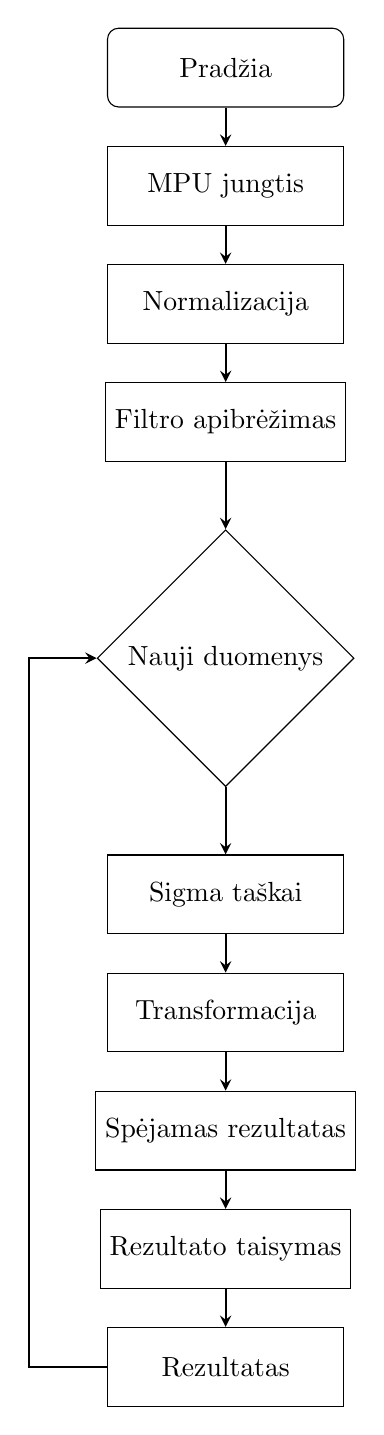
\begin{tikzpicture}[node distance=1.5cm]
        \node (start) [startstop] {Pradžia};
        
        \node (connecttompu) [process, below of=start] {MPU jungtis};
        \node (normalizempu) [process, below of=connecttompu] {Normalizacija};
        
        \node (kalmaninit) [process, below of=normalizempu] {Filtro apibrėžimas};
        \node (newsample) [decision, below of=kalmaninit, yshift=-1.5cm] {Nauji duomenys};

        \node (sigmapoints) [process, below of=newsample, yshift=-1.5cm] {Sigma taškai};
        \node (transform) [process, below of=sigmapoints] {Transformacija};
        \node (kalmanprediction) [process, below of=transform] {Spėjamas rezultatas};
        \node (kalmanupdate) [process, below of=kalmanprediction] {Rezultato taisymas};
        \node (correction) [process, below of=kalmanupdate] {Rezultatas};

        \draw [arrow] (start) -- (connecttompu);
        \draw [arrow] (connecttompu) -- (normalizempu);
        \draw [arrow] (normalizempu) -- (kalmaninit);
        \draw [arrow] (kalmaninit) -- (newsample);
        \draw [arrow] (newsample) -- (sigmapoints);
        \draw [arrow] (sigmapoints) -- (transform);
        \draw [arrow] (transform) -- (kalmanprediction);
        \draw [arrow] (kalmanprediction) -- (kalmanupdate);
        \draw [arrow] (kalmanupdate) -- (correction);

        \draw [arrow] (correction) -- ++(-2.5cm,0) |- (newsample);
    \end{tikzpicture}
\end{figure}


\end{document}
